\chapter{Fits}

\section{\unit{36}{\invpb}}

\begin{figure}
\begin{center}
% bottom right top left
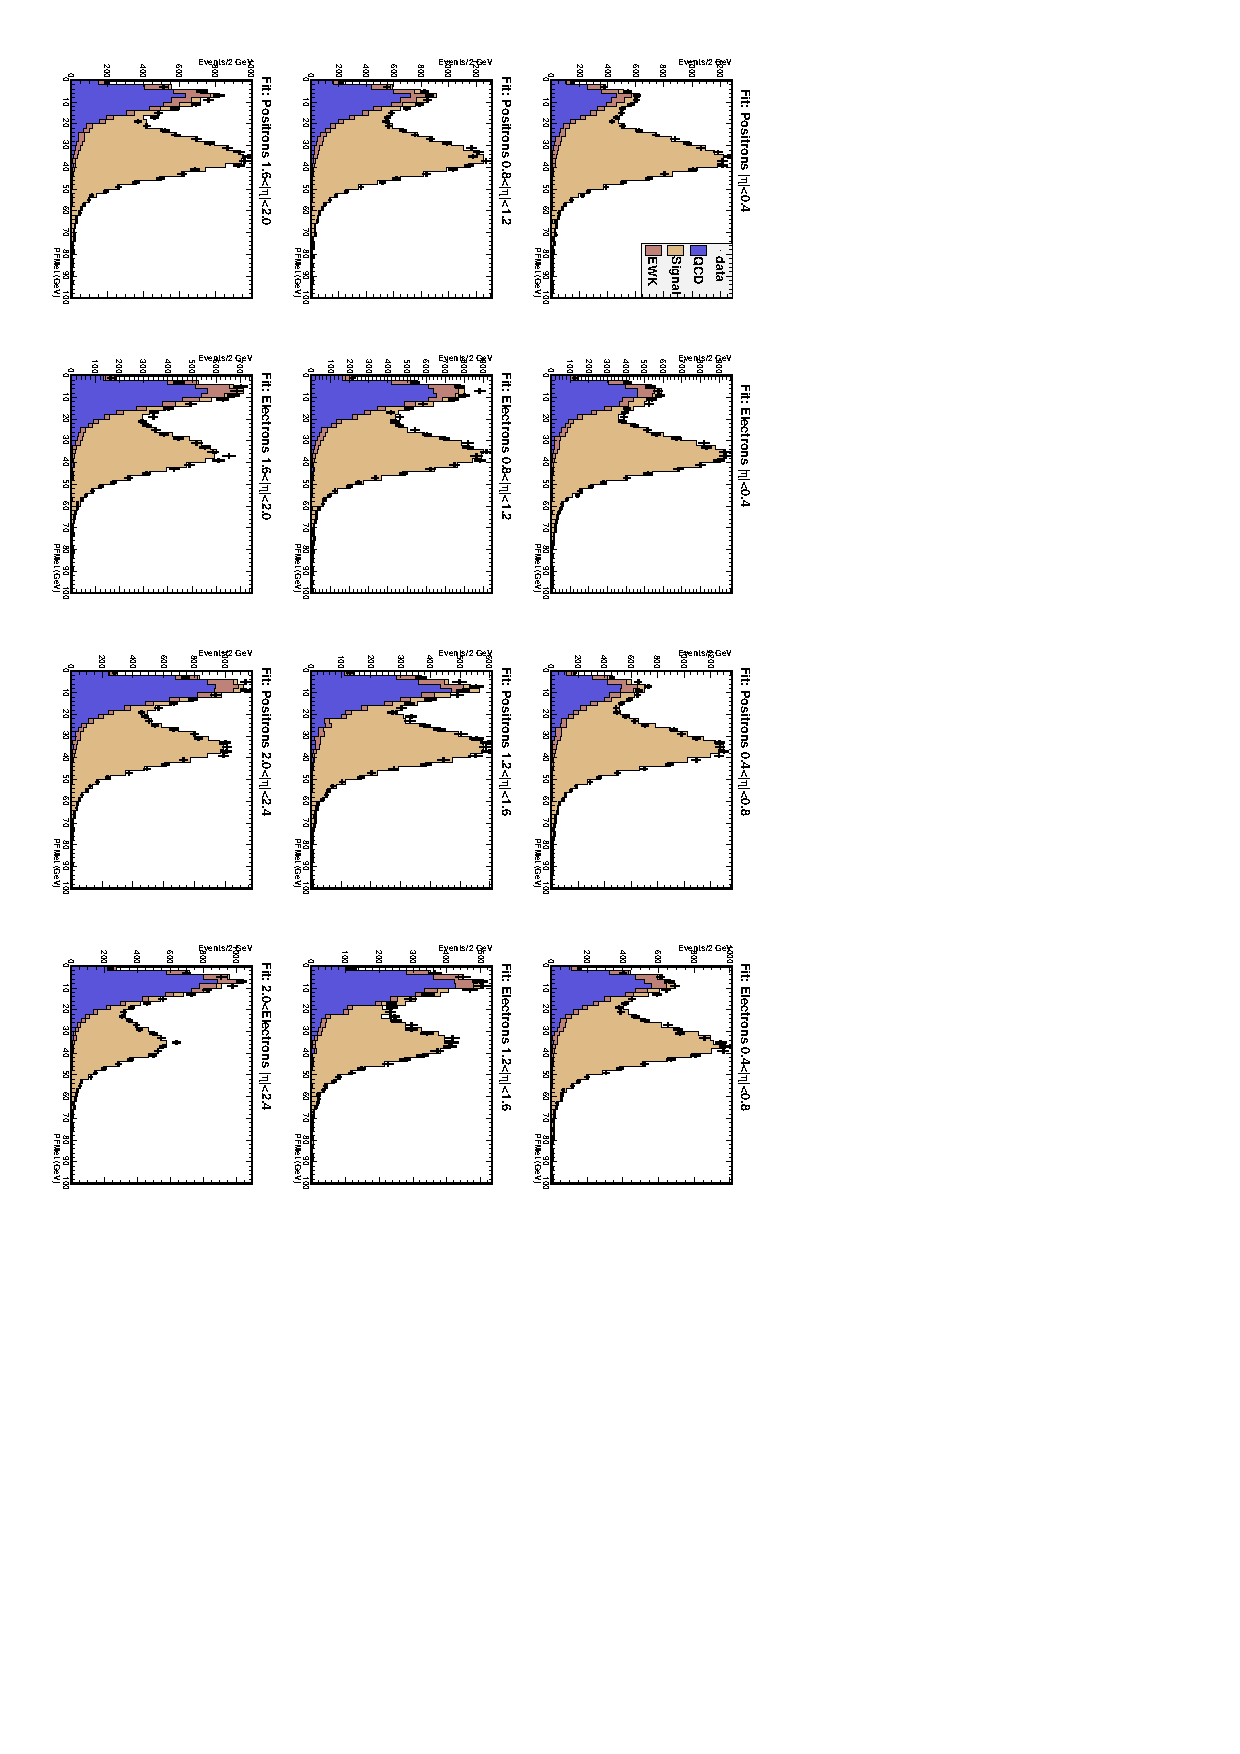
\includegraphics[trim = 80mm 100mm 0mm 0mm, clip, angle=90, width=0.95\textwidth]{Dec22_data}
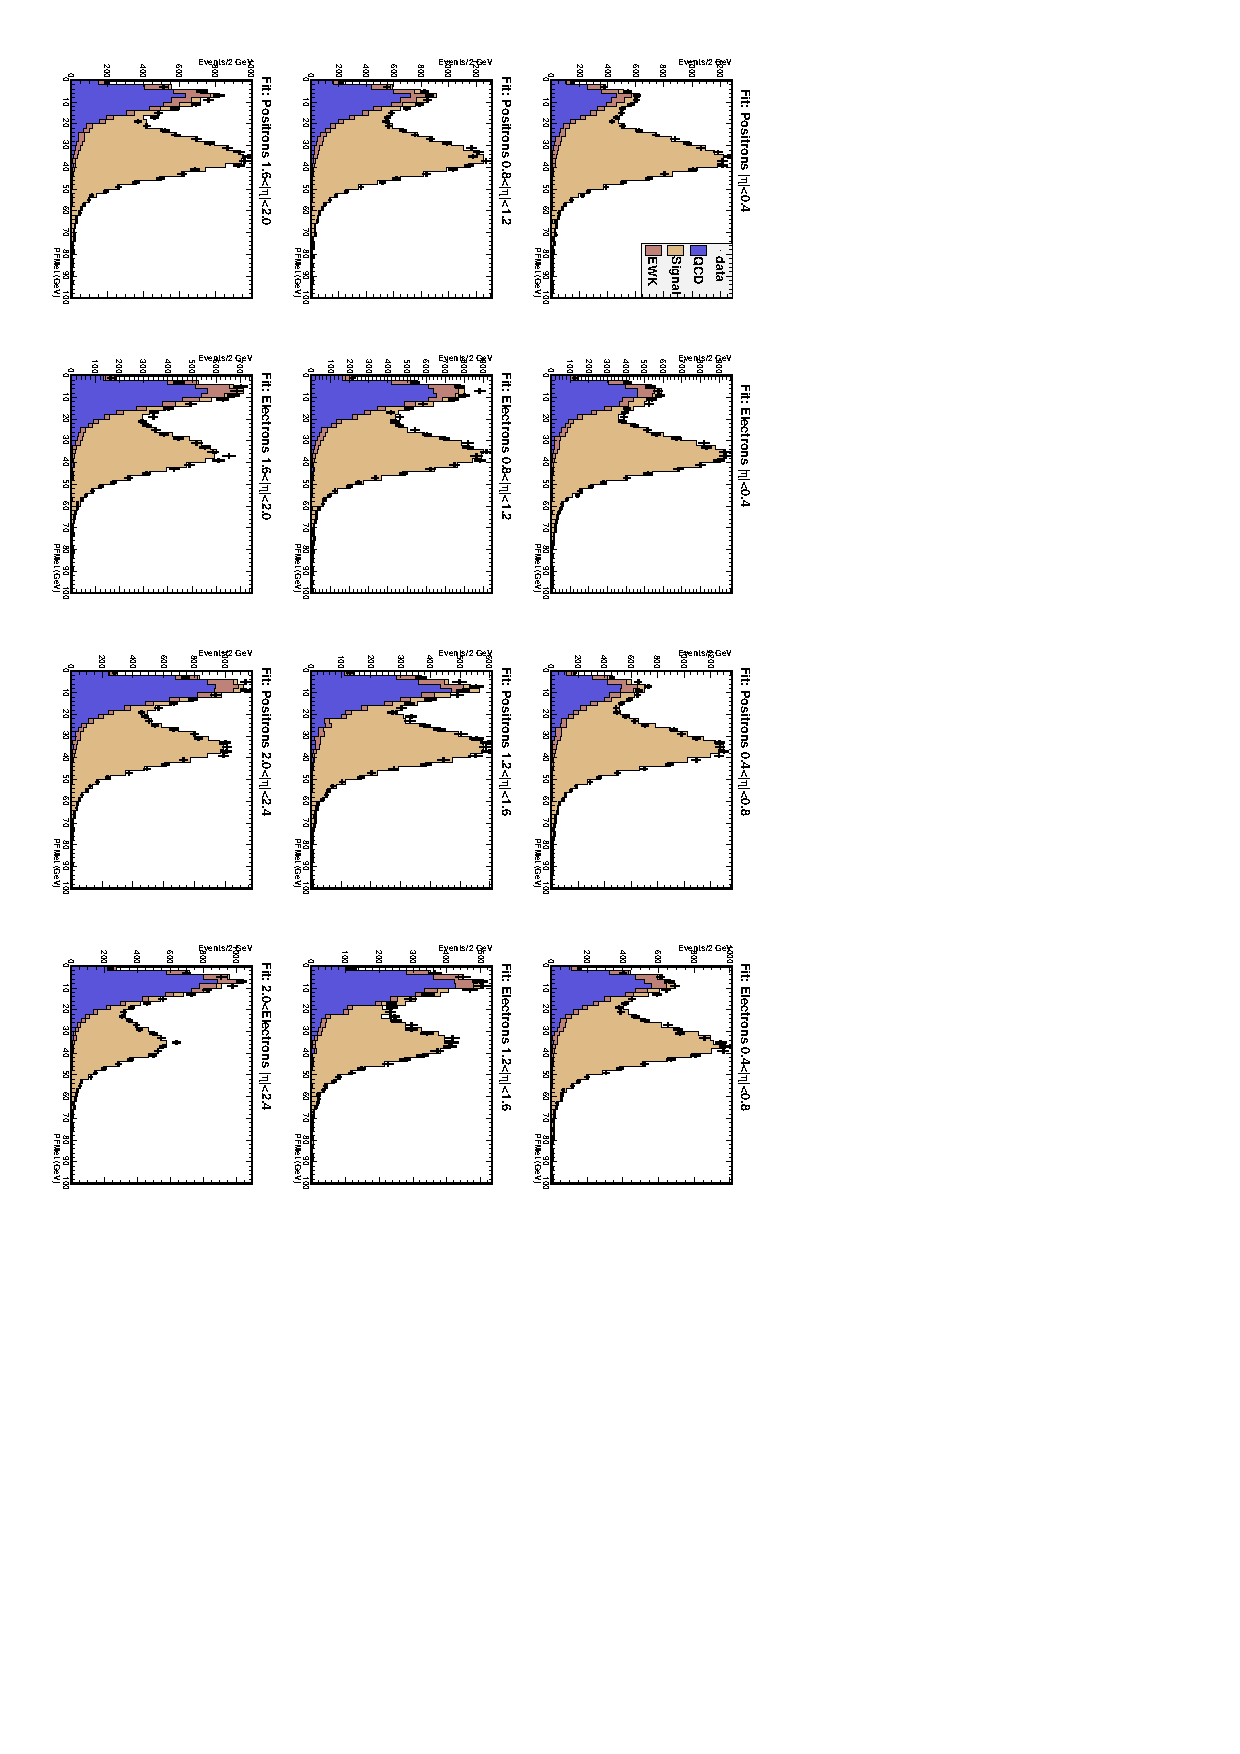
\includegraphics[trim = 80mm 0mm 0mm 100mm, clip, angle=90, width=0.95\textwidth]{Dec22_data}
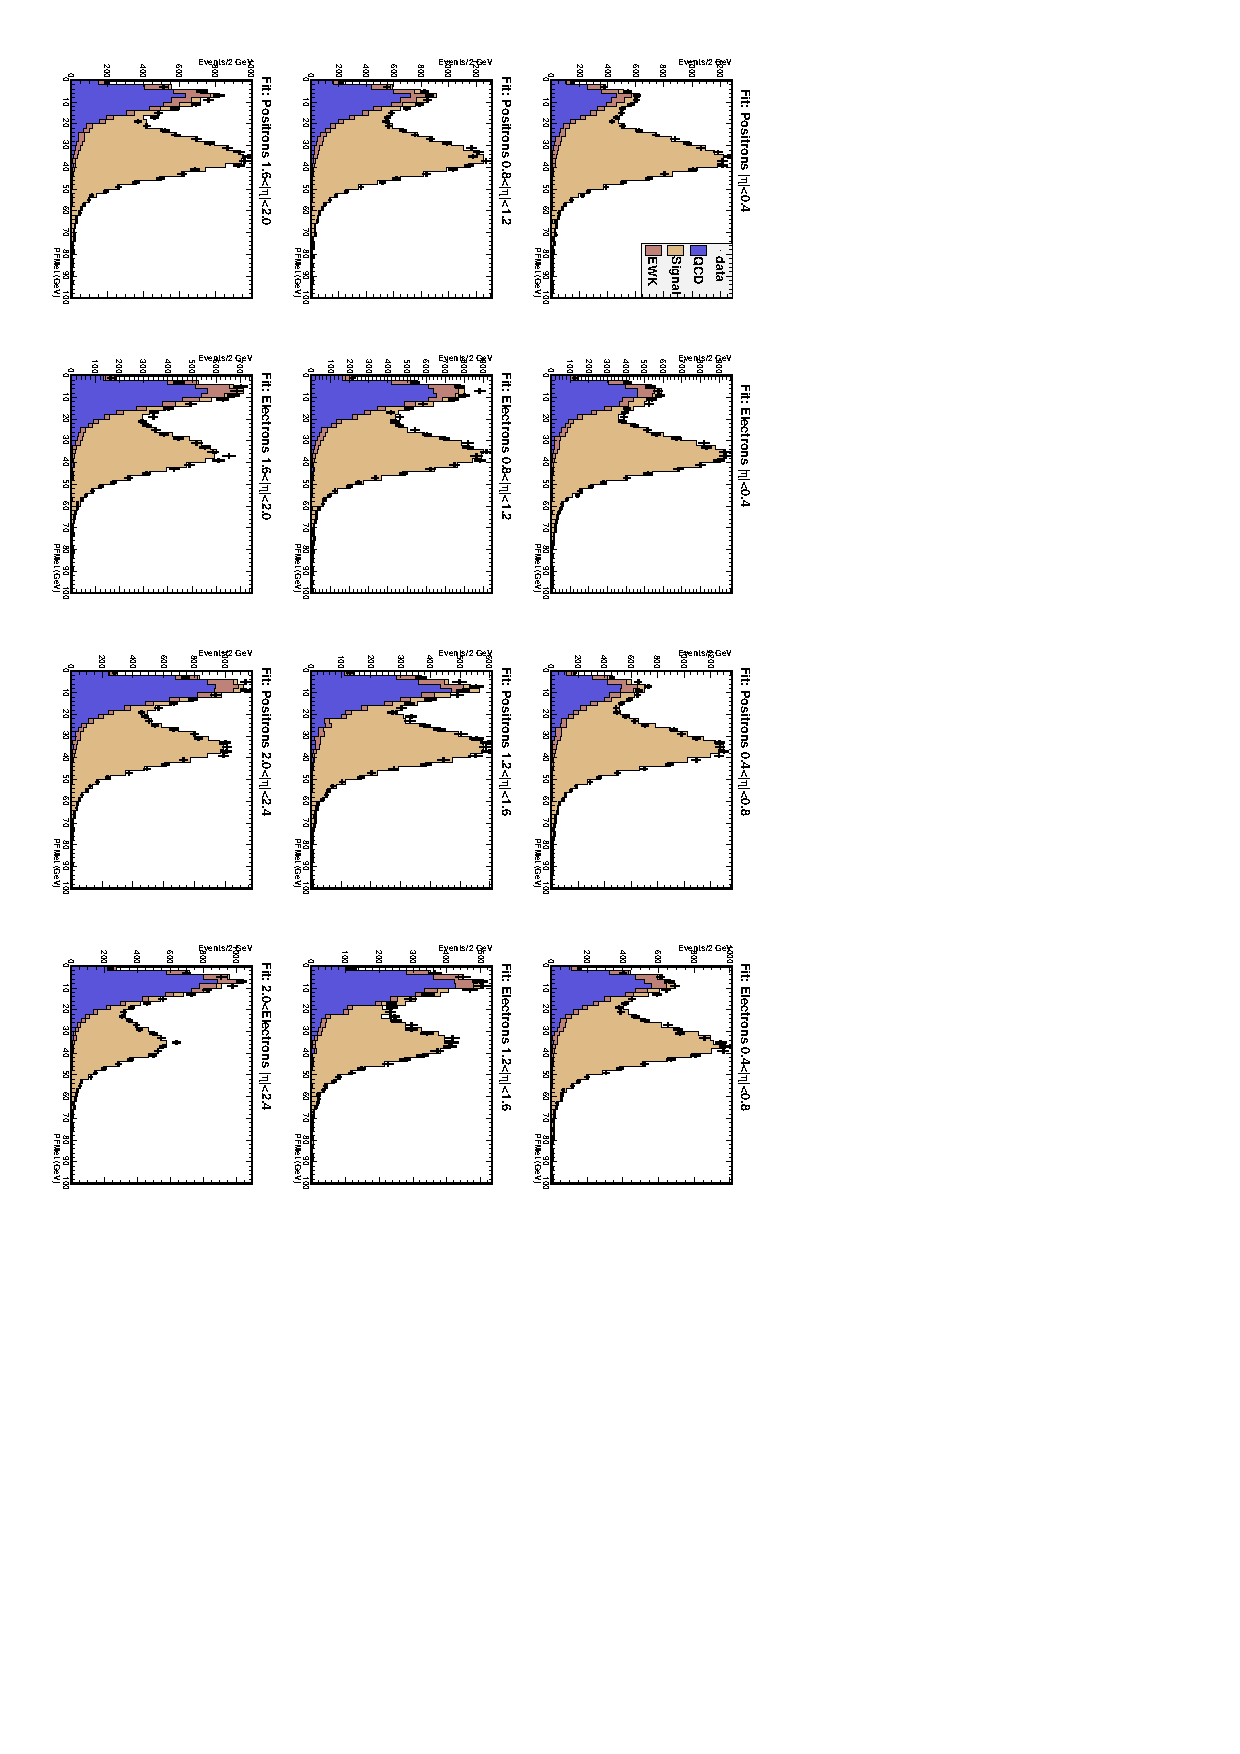
\includegraphics[trim = 40mm 100mm 40mm 0mm, clip, angle=90, width=0.95\textwidth]{Dec22_data}
\caption{  \label{fig:fit1} The fit to \ETm\ for each pseudorapidity/charge
bin.  The $x$-axis is the particle flow \ETm (GeV) and the $y$-axis is the
number of events ($2\GeV^{-1}$).}
\end{center}
\end{figure}

\begin{figure}
\begin{center}
% bottom right top left
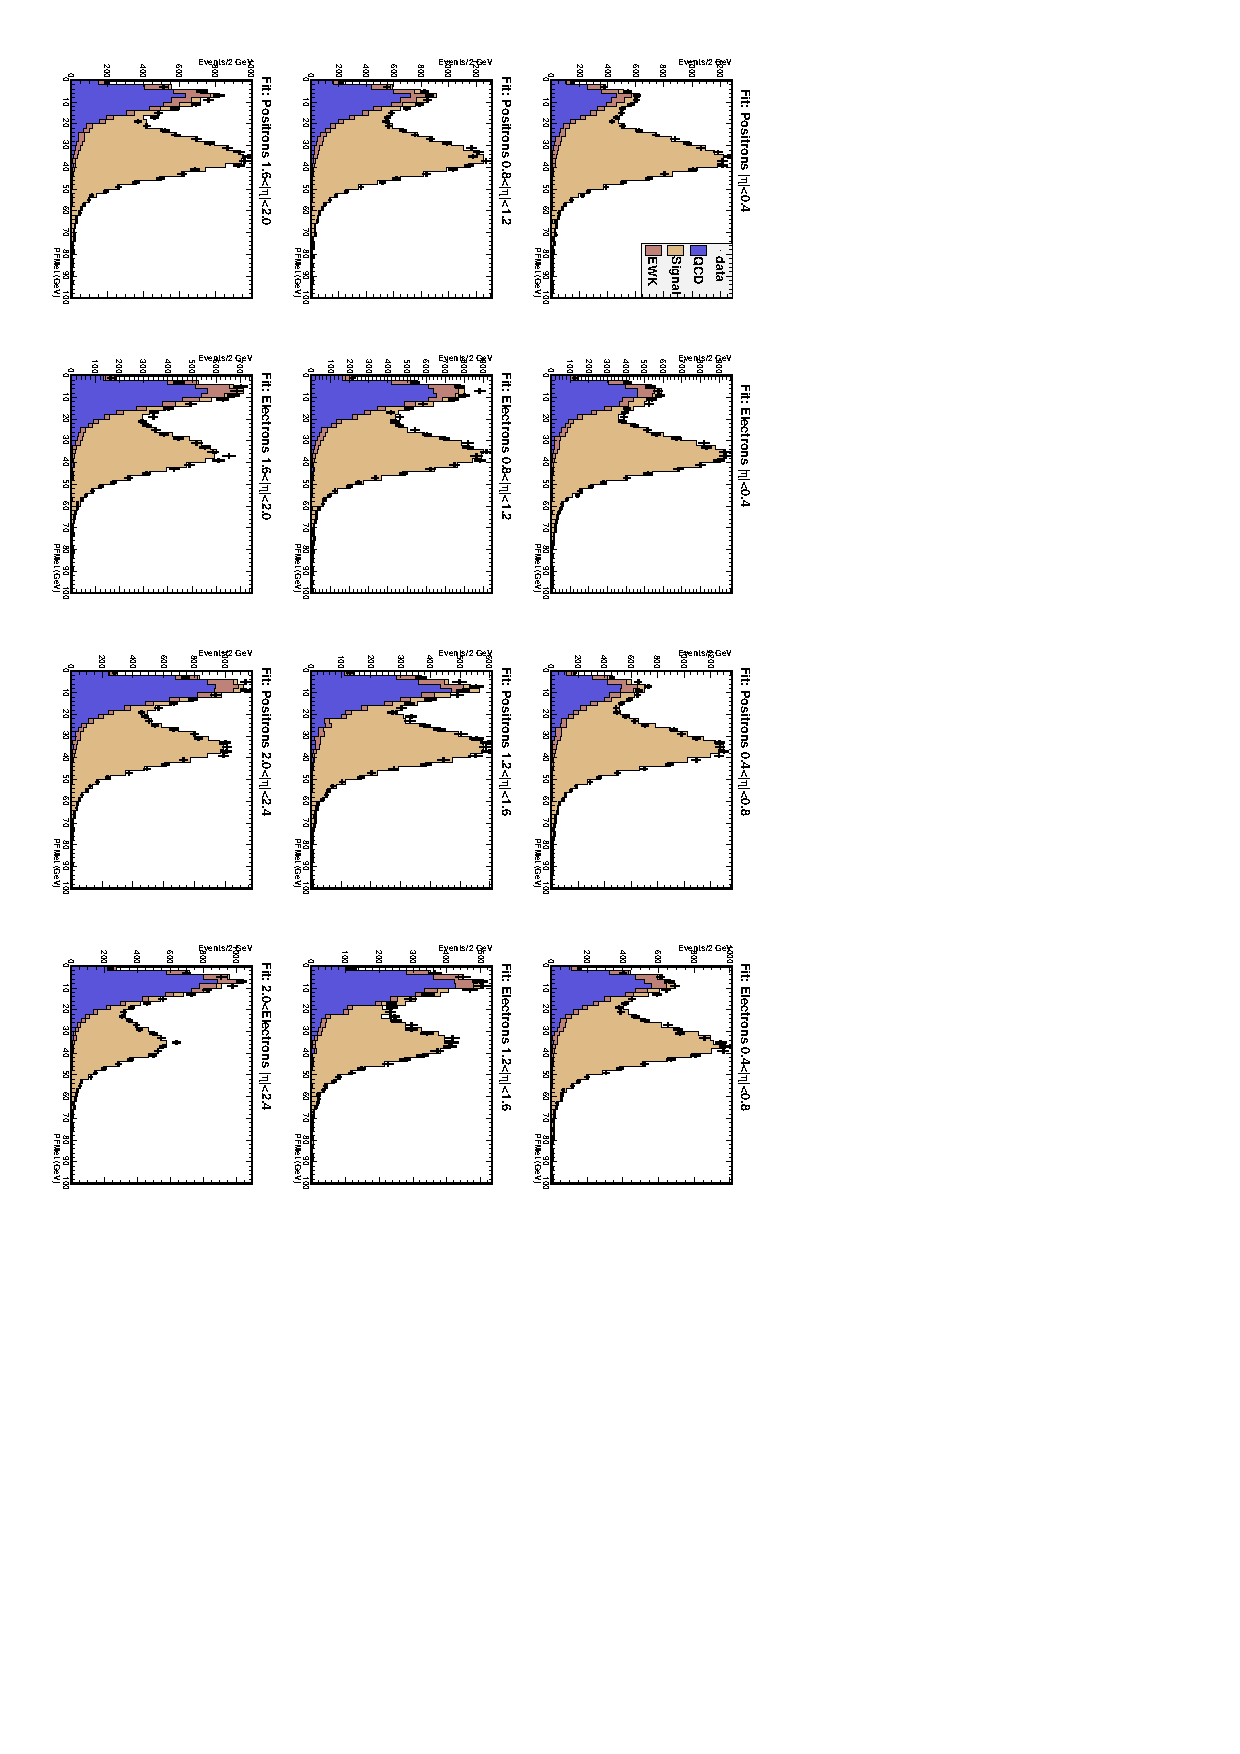
\includegraphics[trim = 40mm 0mm 40mm 100mm, clip, angle=90, width=0.95\textwidth]{Dec22_data}
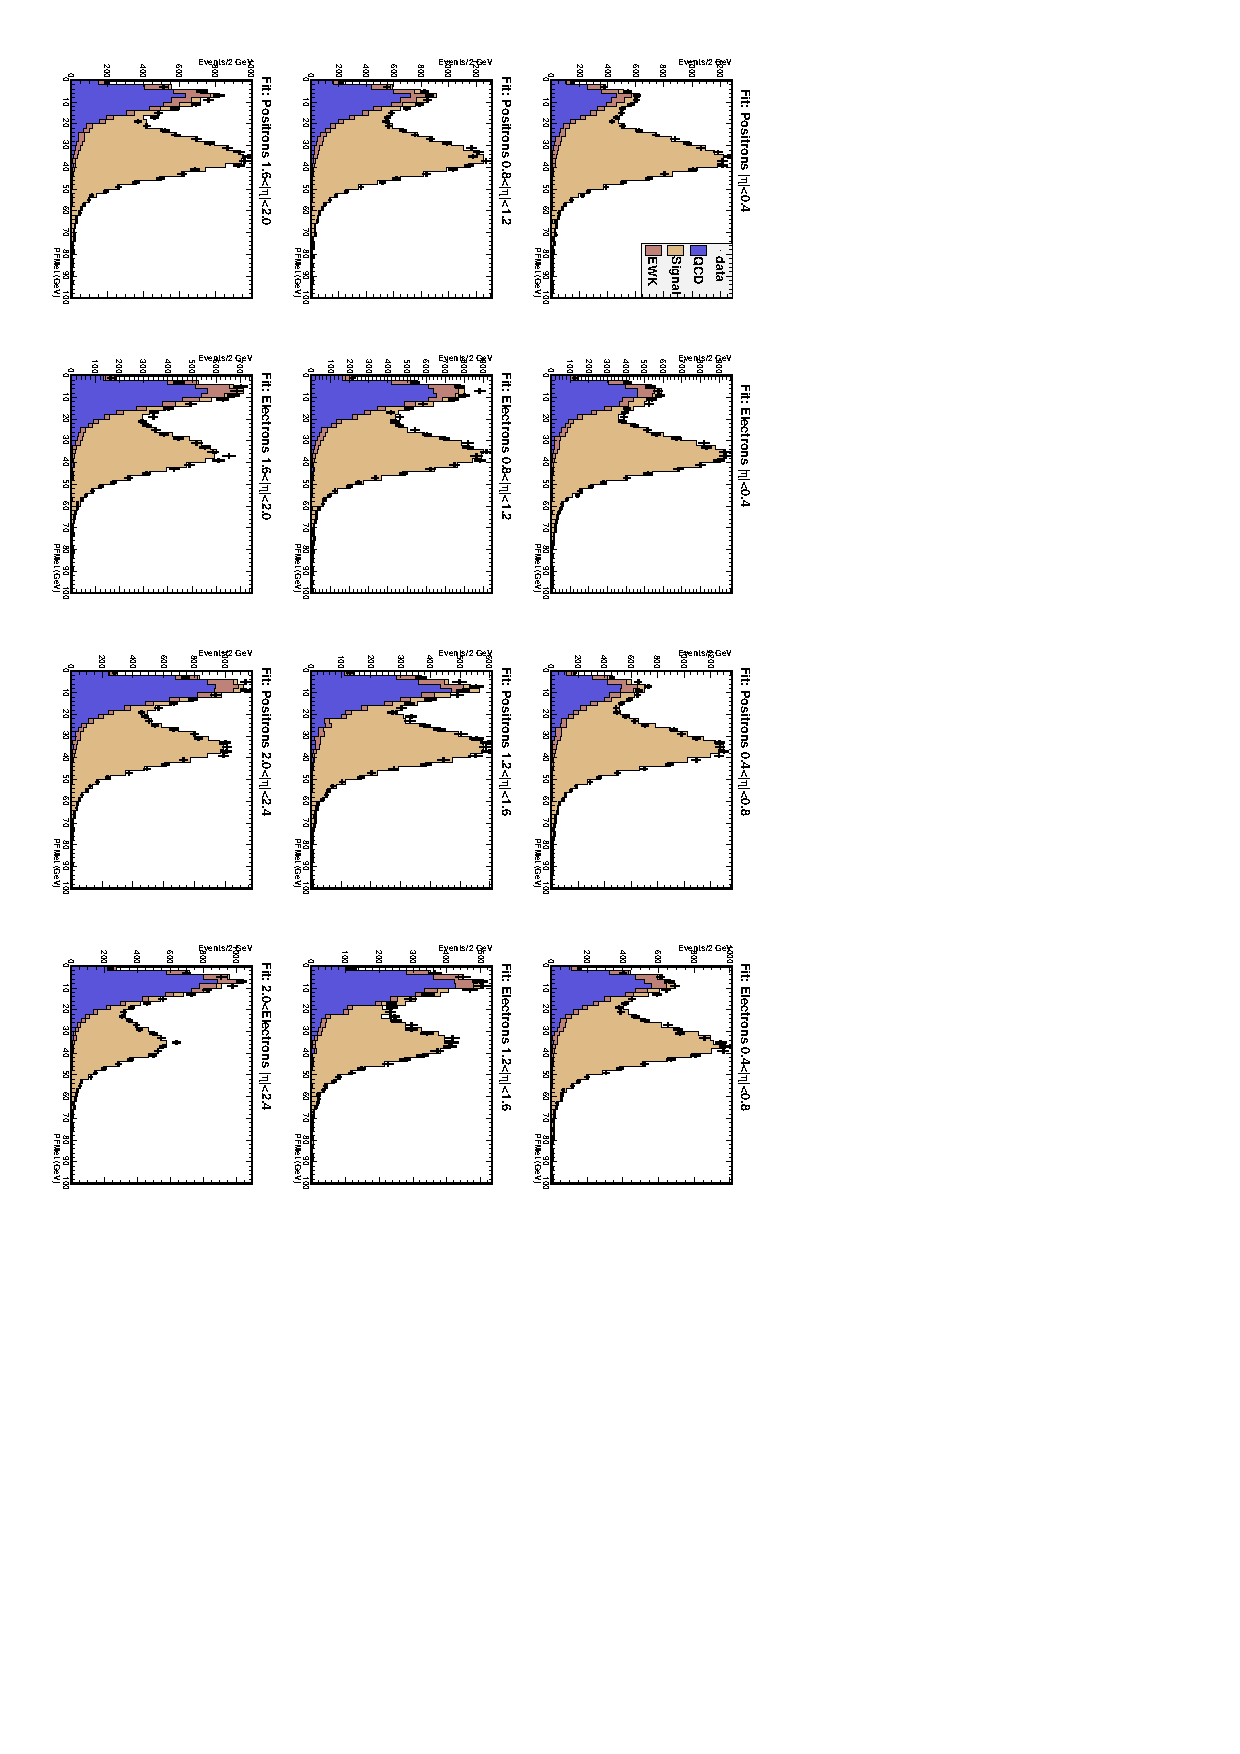
\includegraphics[trim = 0mm 100mm 80mm 0mm, clip, angle=90, width=0.95\textwidth]{Dec22_data}
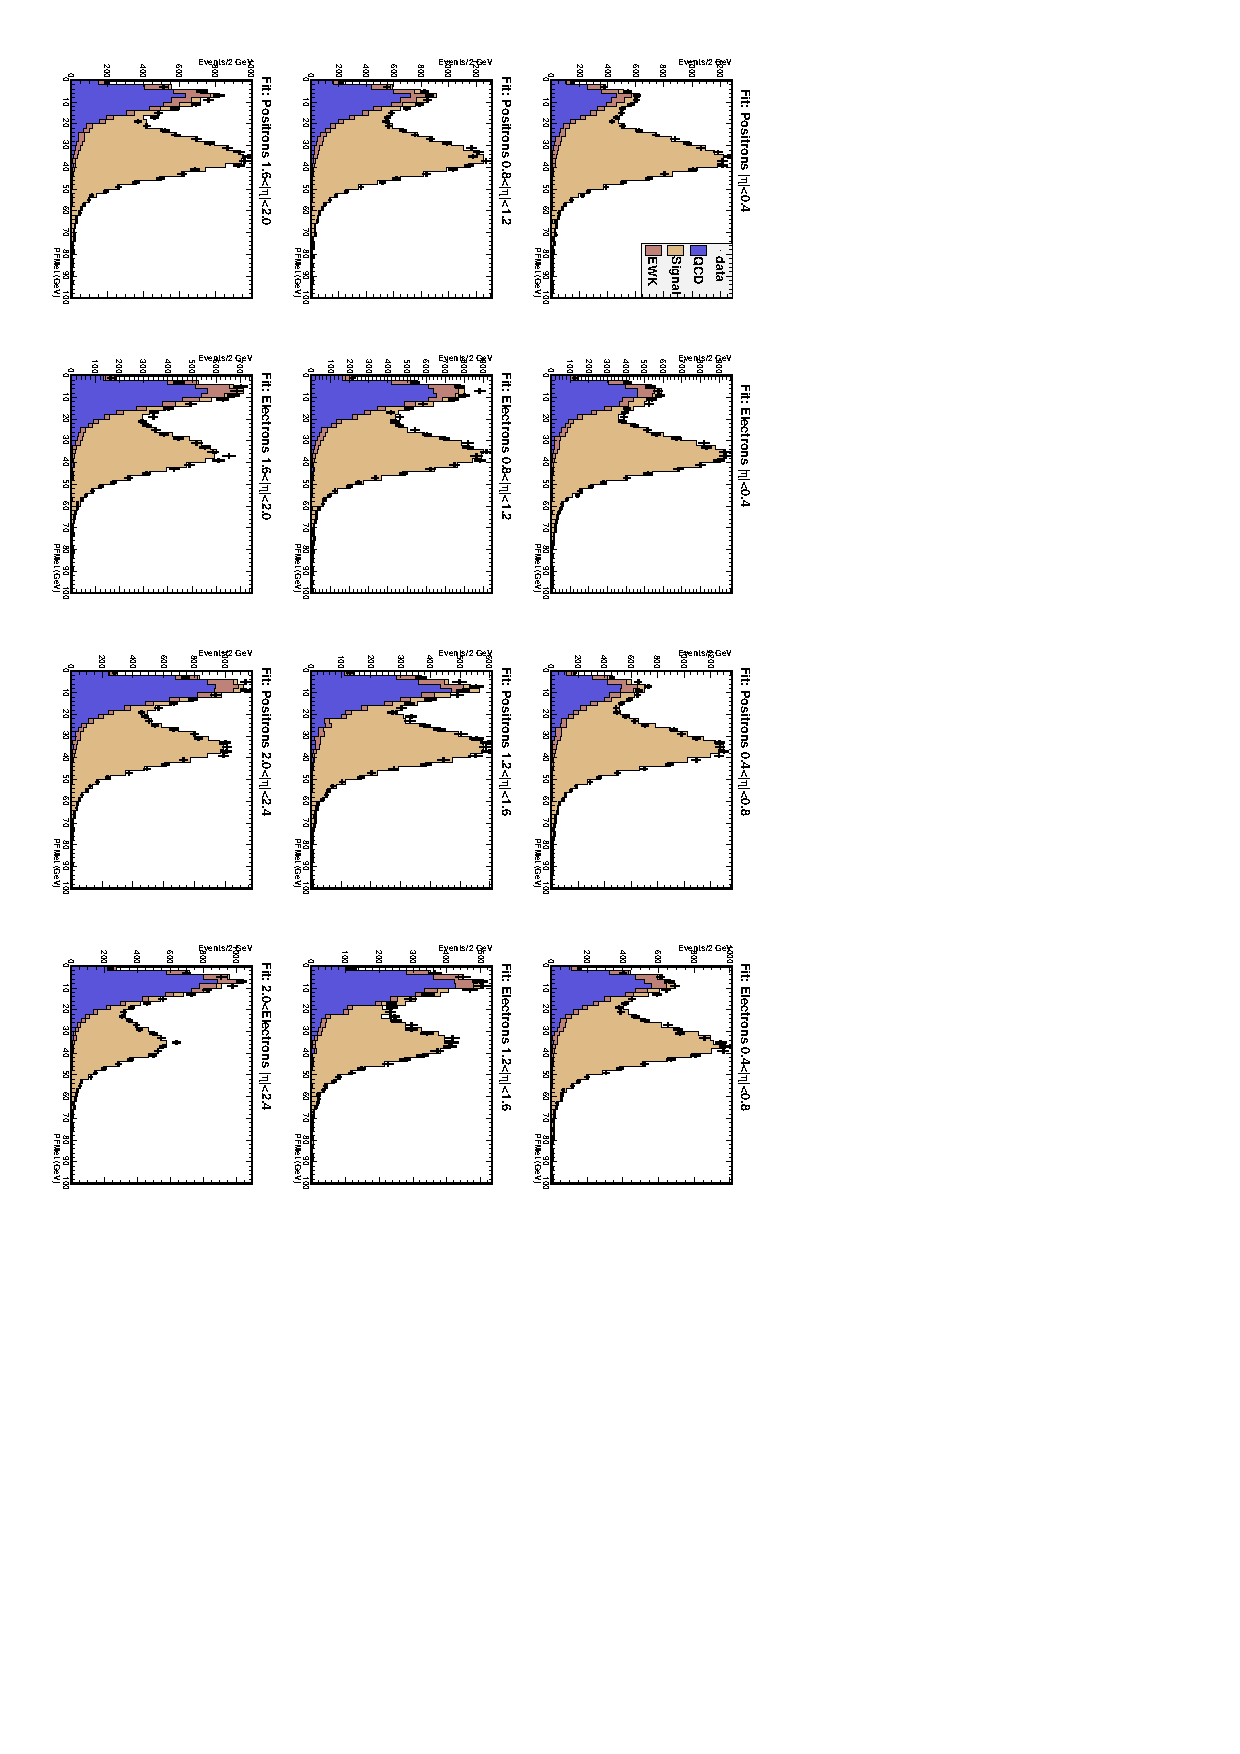
\includegraphics[trim = 0mm 0mm 80mm 100mm, clip, angle=90, width=0.95\textwidth]{Dec22_data}
\caption{  \label{fig:fit2} The fit to \ETm\ for each pseudorapidity/charge
bin.  The $x$-axis is the particle flow \ETm (GeV) and the $y$-axis is the
number of events ($2\GeV^{-1}$).}
\end{center}
\end{figure}

\begin{figure}
\begin{center}
% bottom right top left
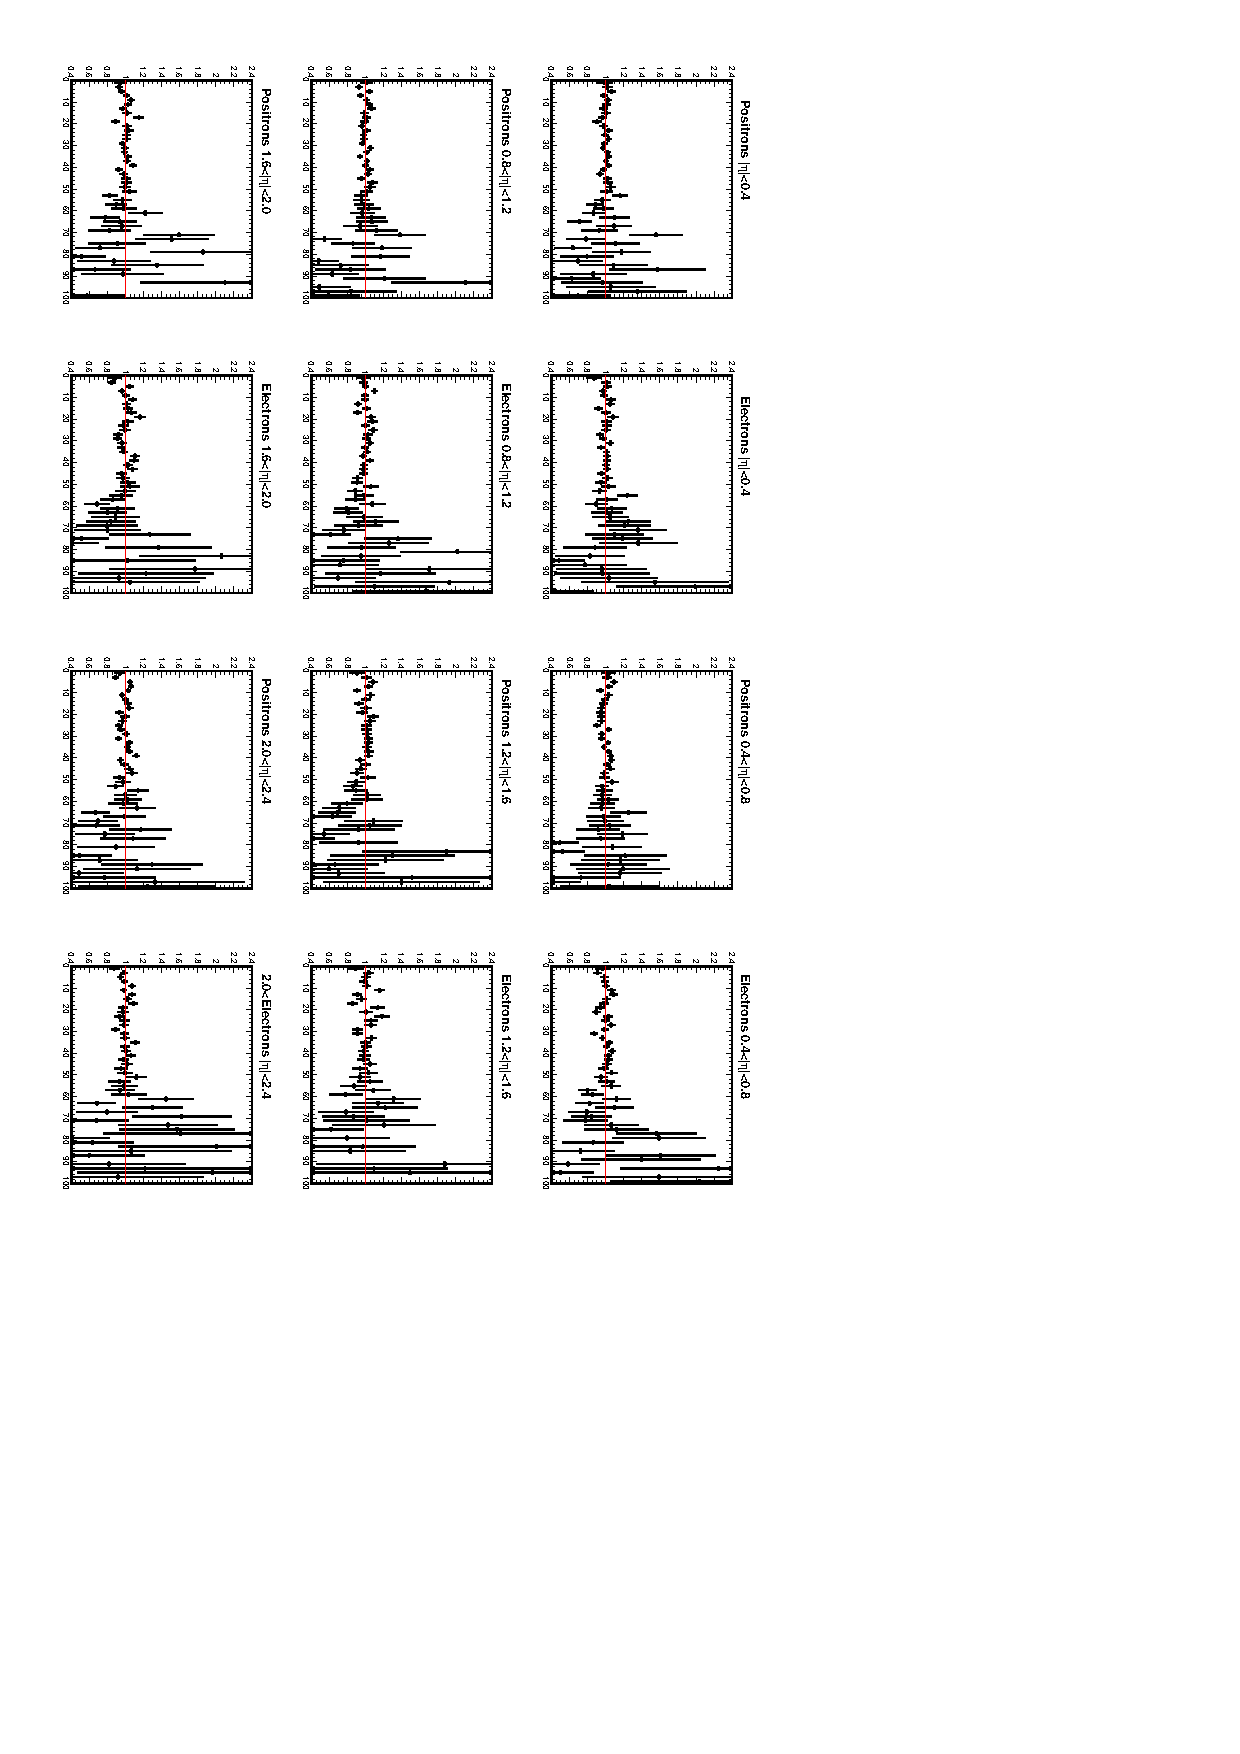
\includegraphics[trim = 80mm 100mm 0mm 0mm, clip, angle=90, width=0.95\textwidth]{Dec22_fitratio}
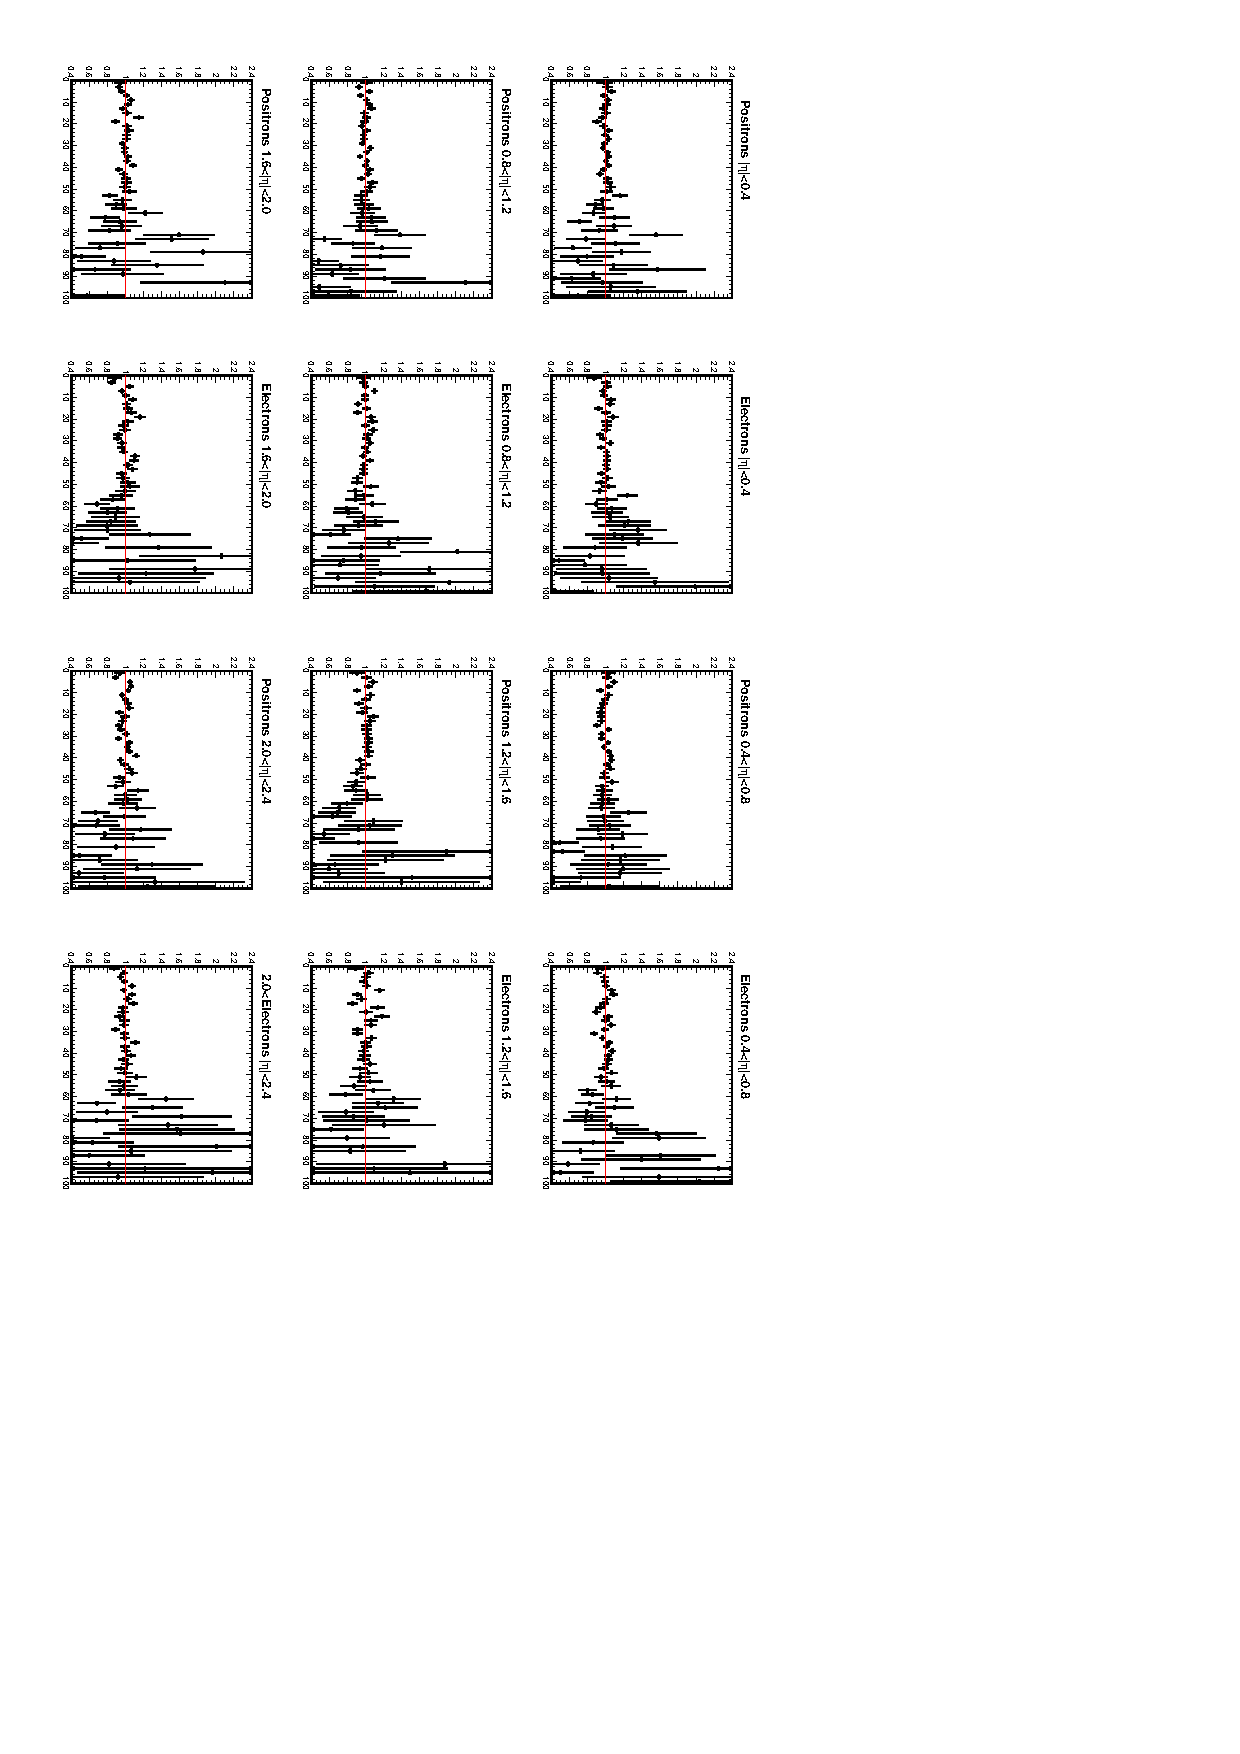
\includegraphics[trim = 80mm 0mm 0mm 100mm, clip, angle=90, width=0.95\textwidth]{Dec22_fitratio}
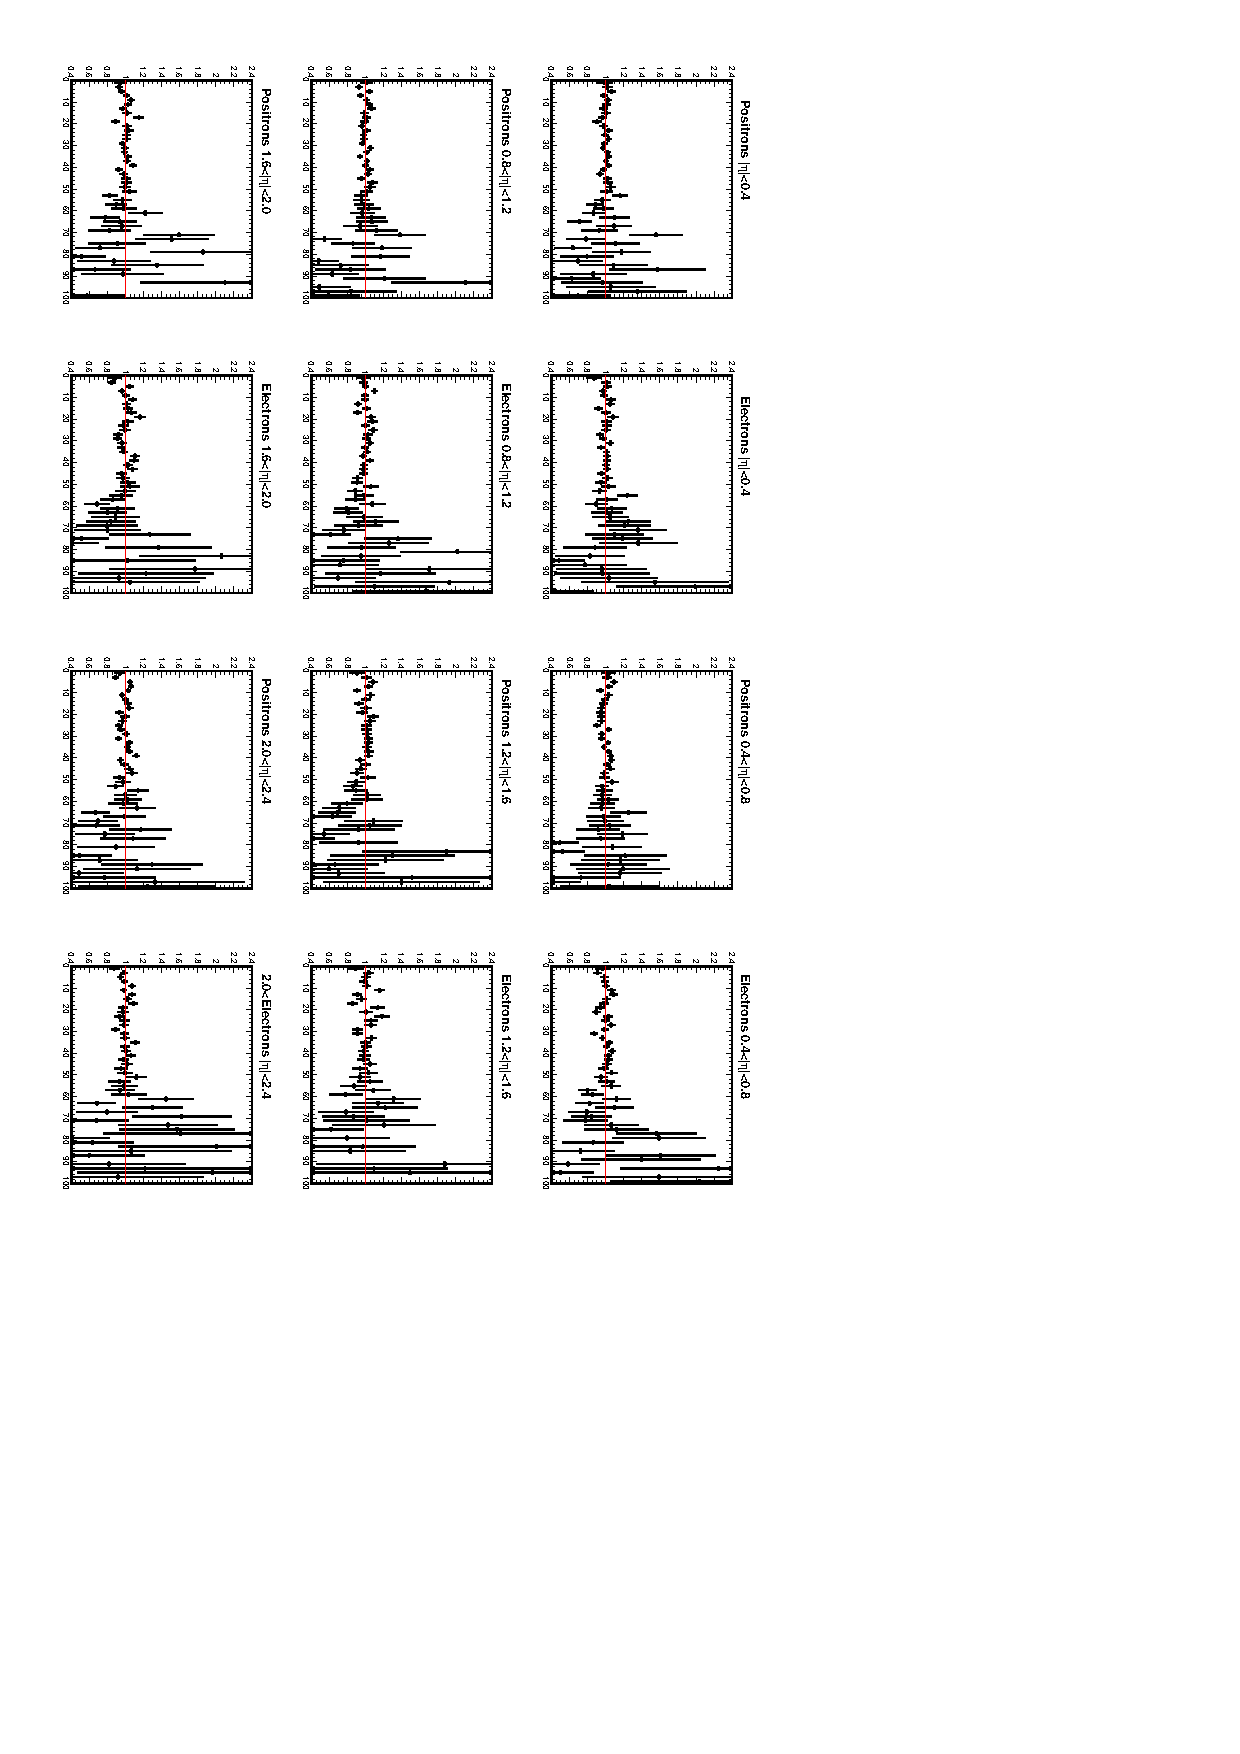
\includegraphics[trim = 40mm 100mm 40mm 0mm, clip, angle=90, width=0.95\textwidth]{Dec22_fitratio}
\caption{\label{fig:fit1ratio}Ratio between fit and data for each pseudorapidity/charge bin.
The $x$-axis is the particle flow \ETm (GeV).}
\end{center}
\end{figure}

\begin{figure}
\begin{center}
% bottom right top left
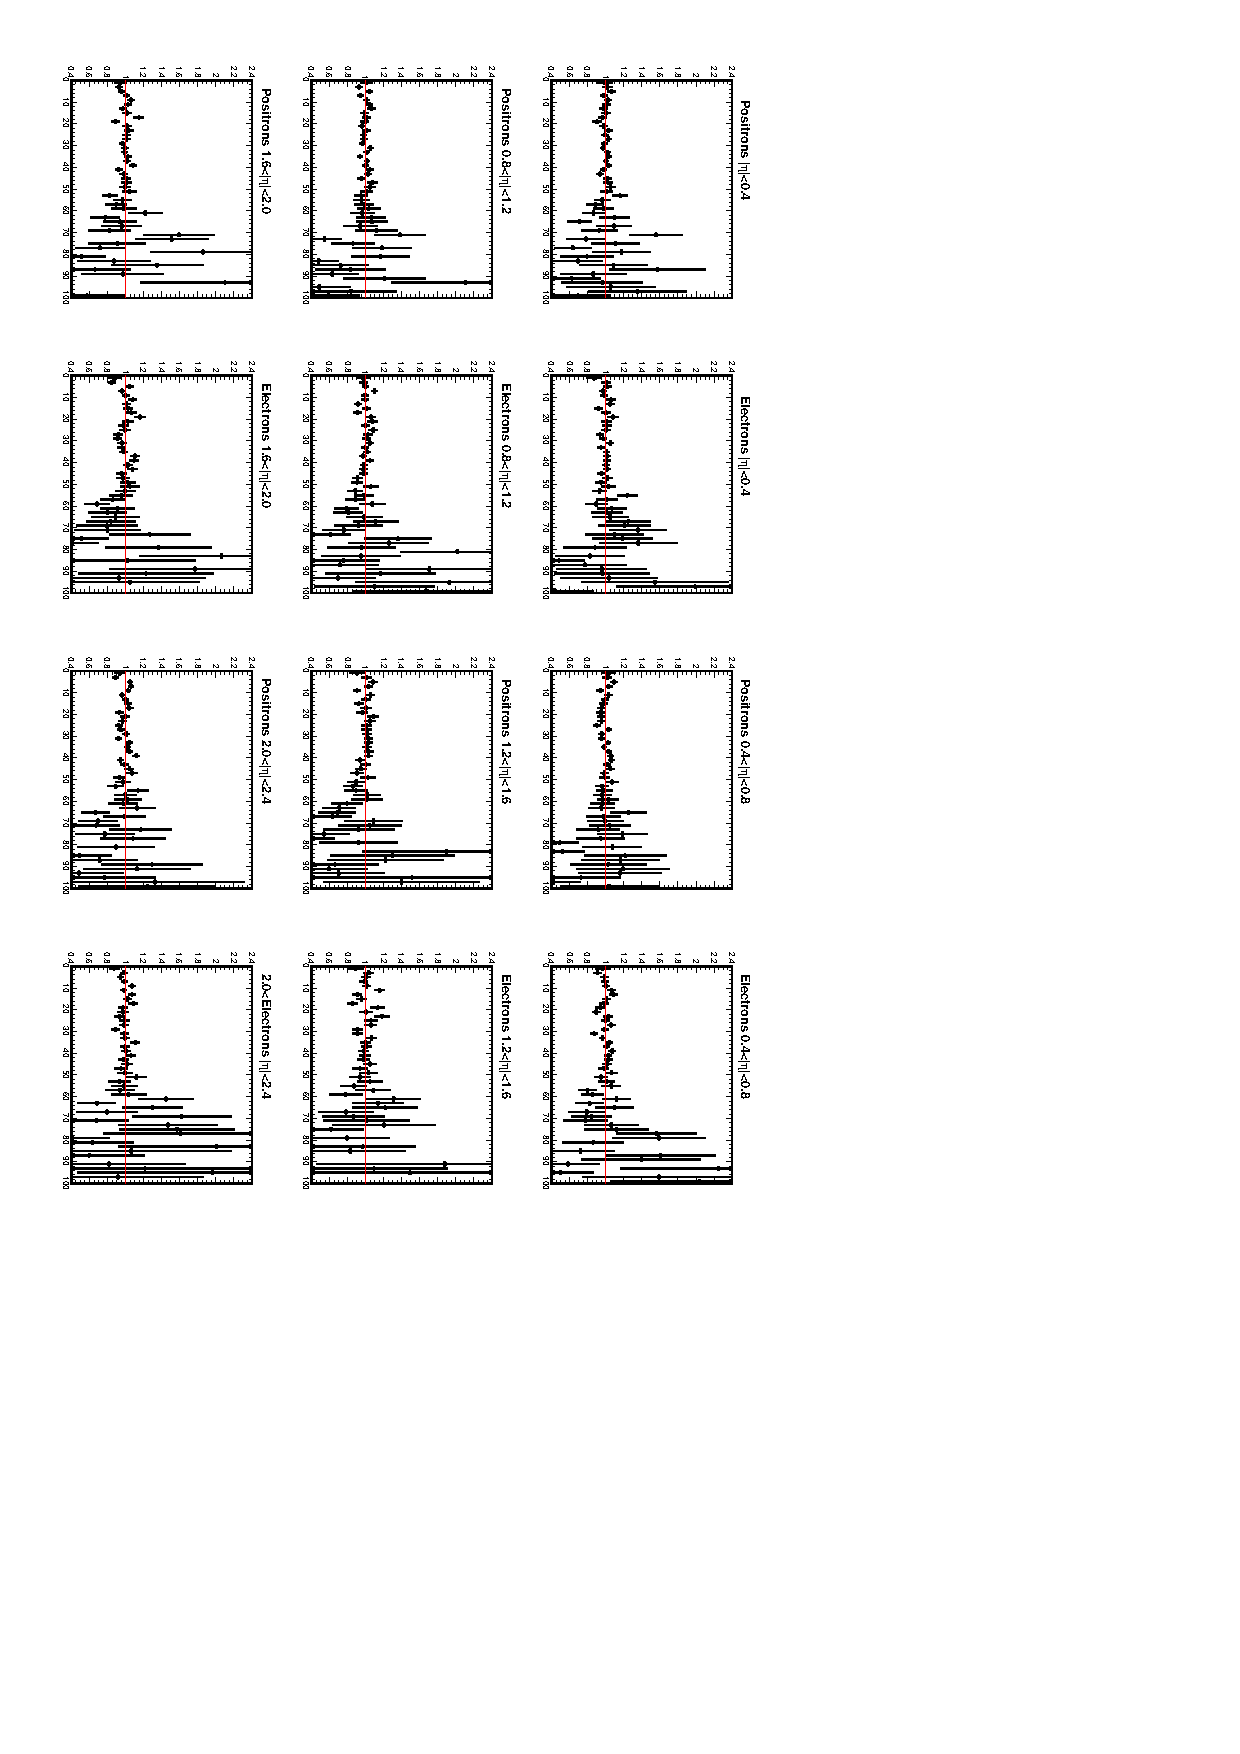
\includegraphics[trim = 40mm 0mm 40mm 100mm, clip, angle=90, width=0.95\textwidth]{Dec22_fitratio}
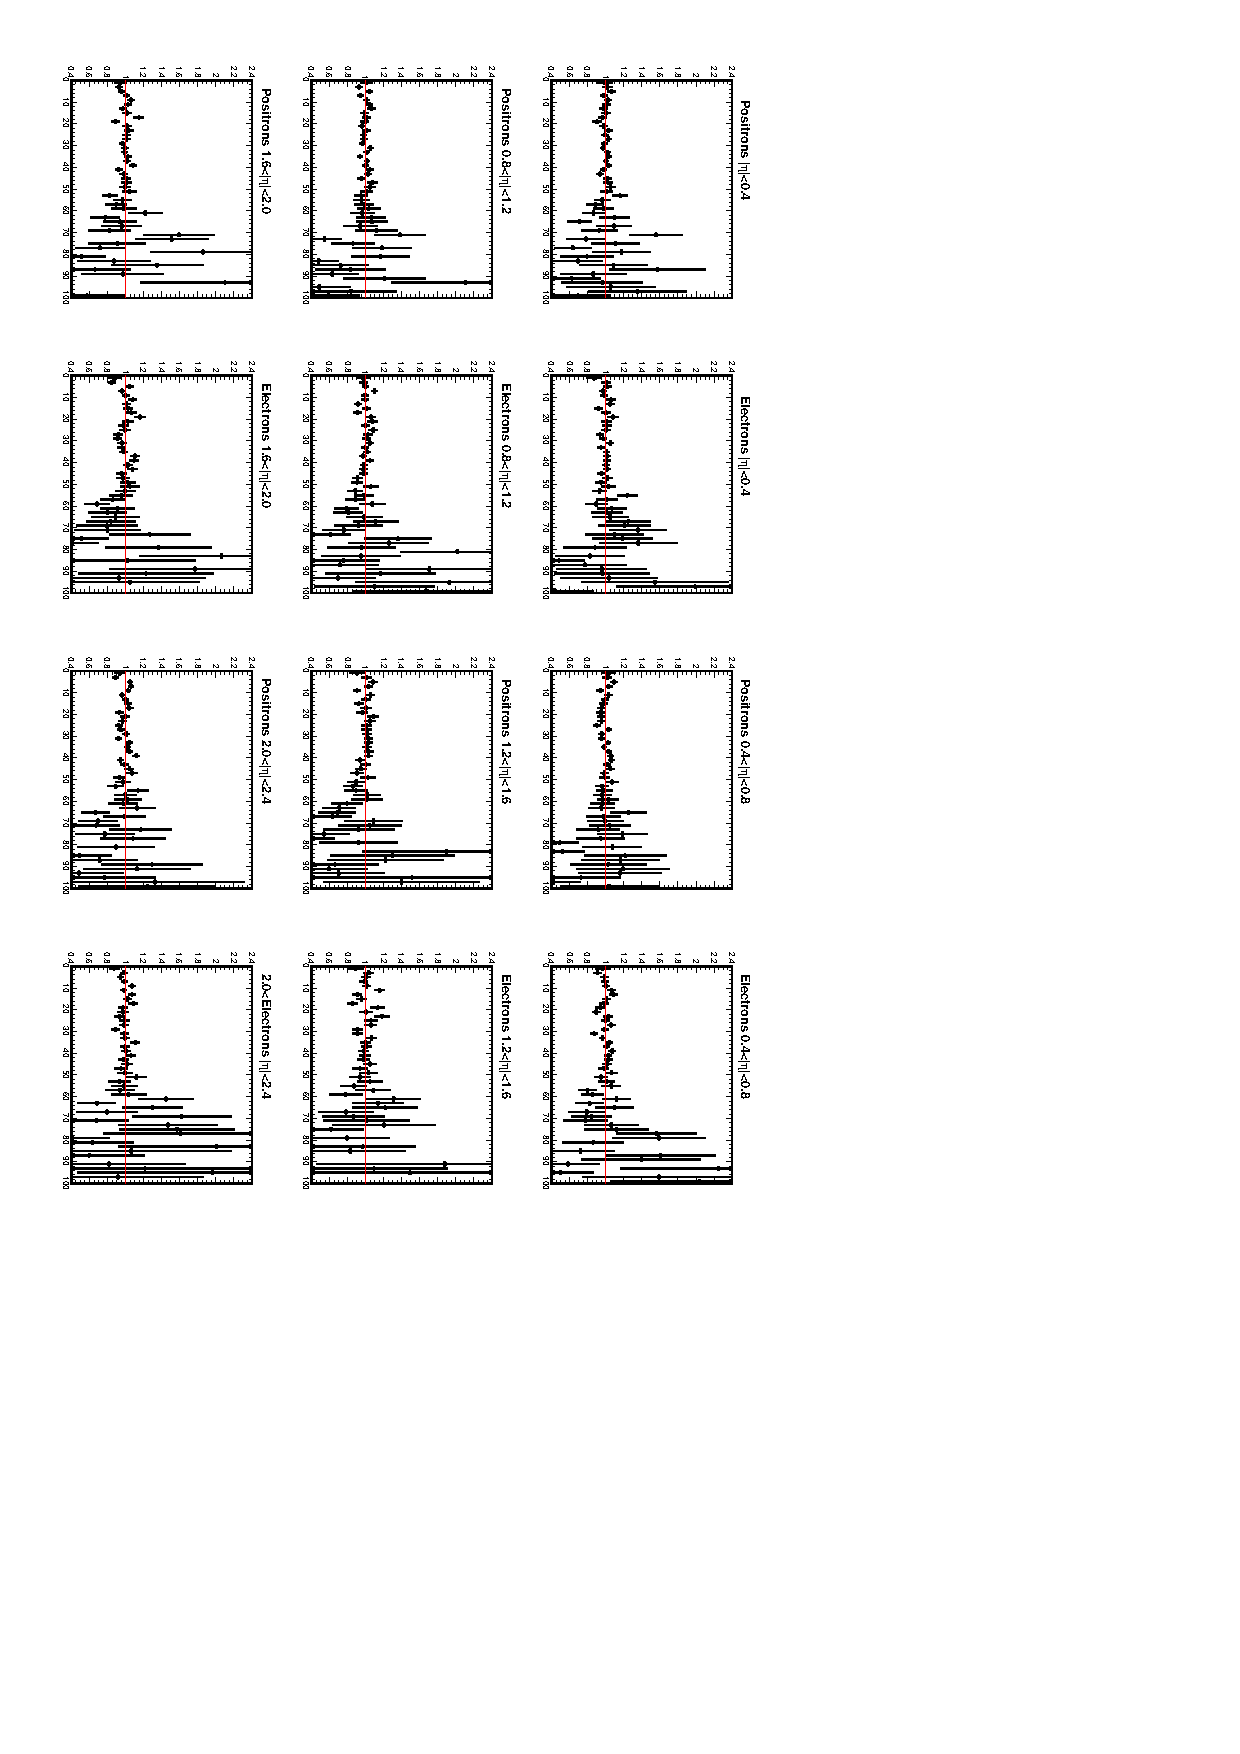
\includegraphics[trim = 0mm 100mm 80mm 0mm, clip, angle=90, width=0.95\textwidth]{Dec22_fitratio}
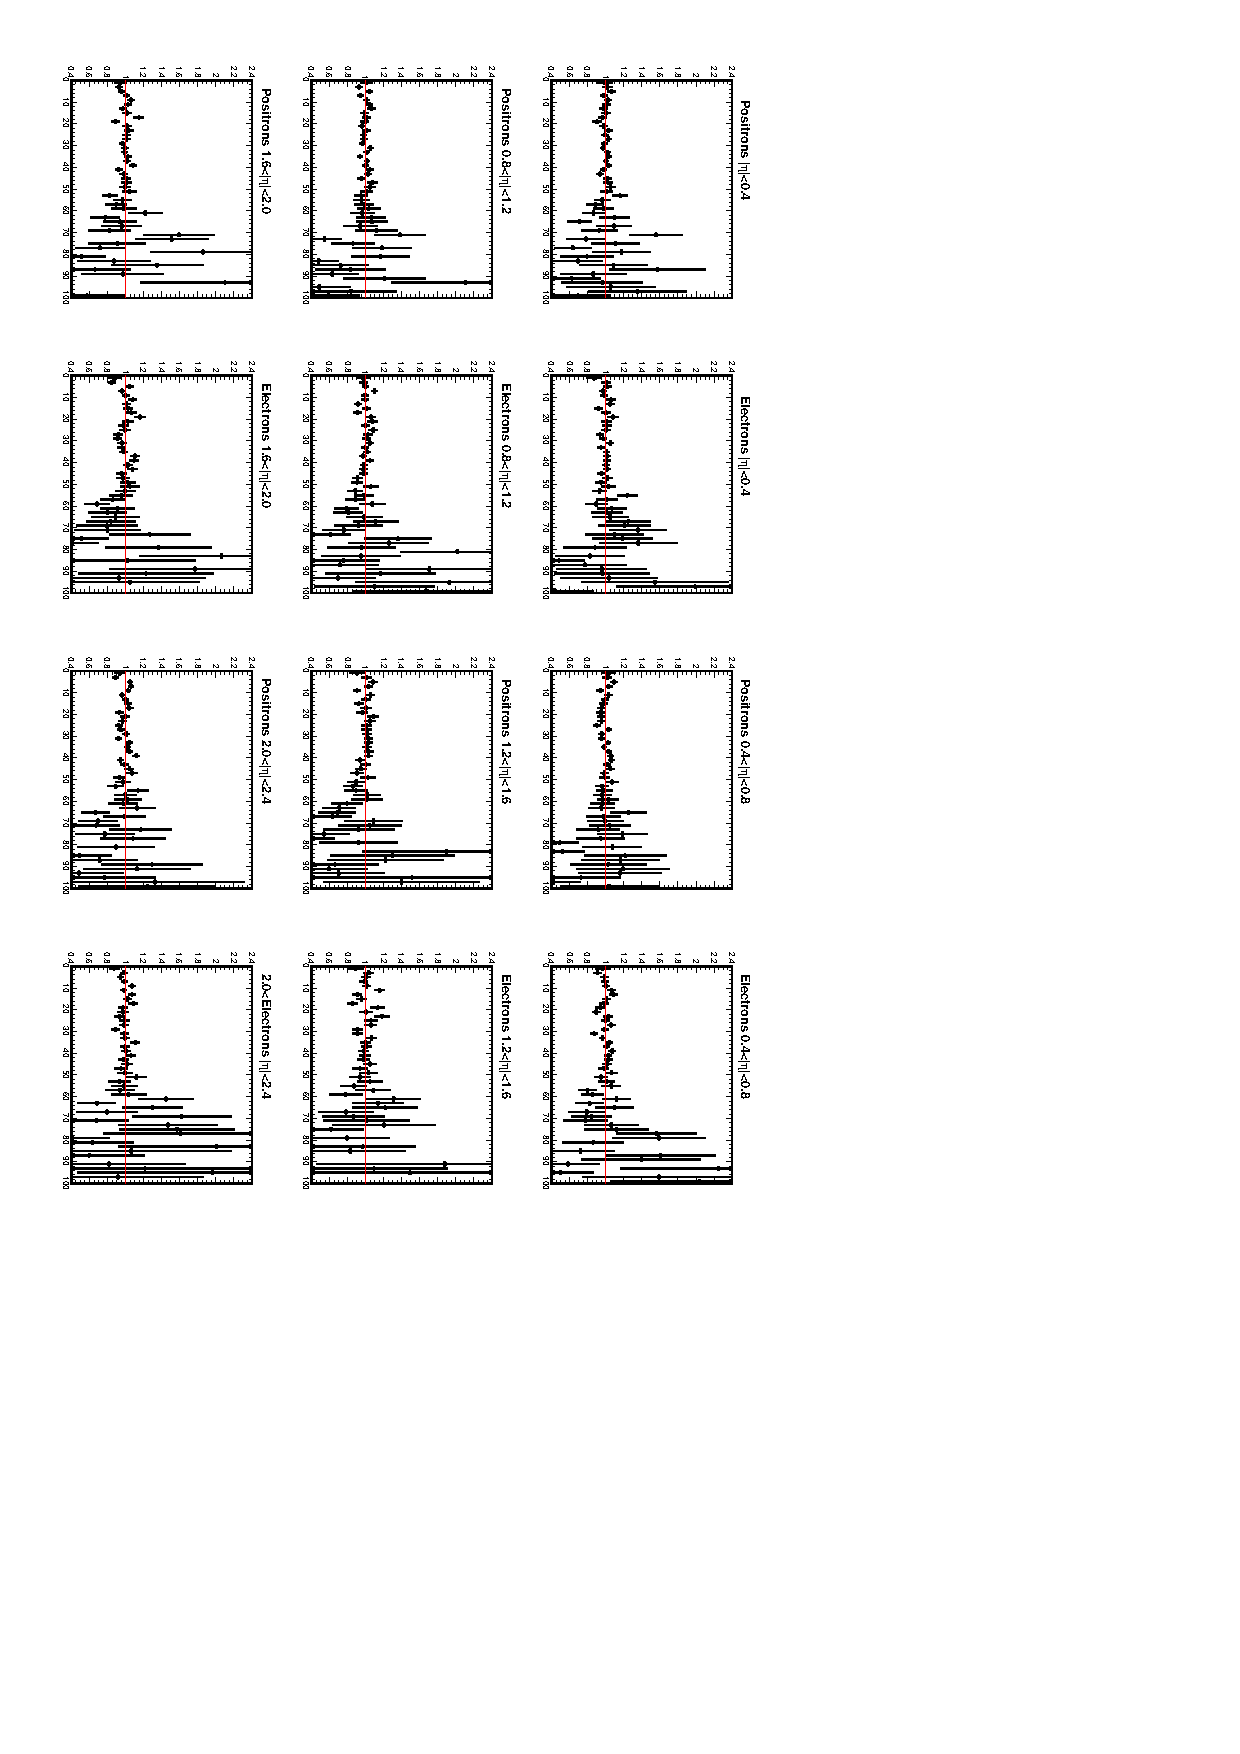
\includegraphics[trim = 0mm 0mm 80mm 100mm, clip, angle=90, width=0.95\textwidth]{Dec22_fitratio}
\caption{\label{fig:fit2ratio}Ratio between fit and data for each
pseudorapidity/charge bin.  The $x$-axis is the particle flow \ETm (GeV).}
\end{center}
\end{figure}

\clearpage

\section{\unit{840}{\invpb}}

\begin{figure}
\begin{center}
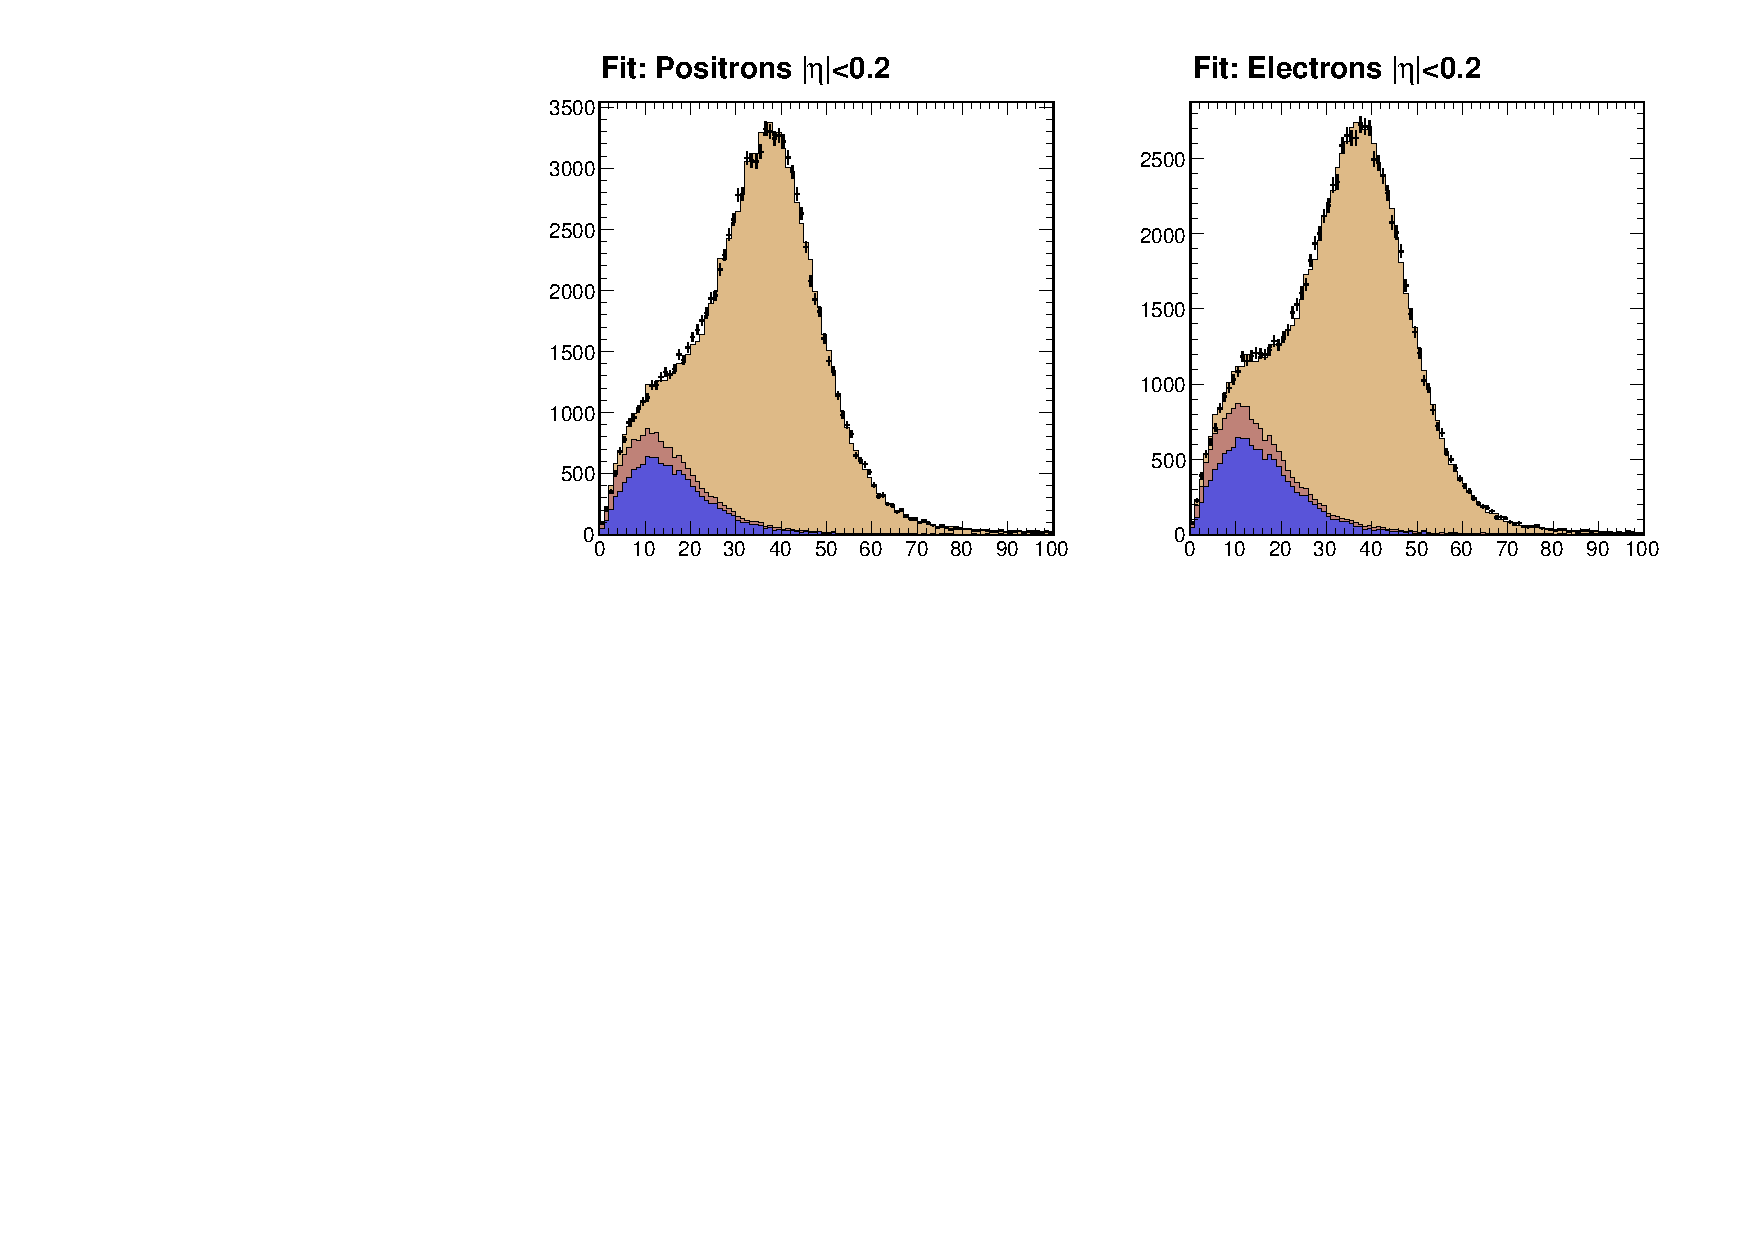
\includegraphics[width=0.95\textwidth]{data_0.pdf} \\
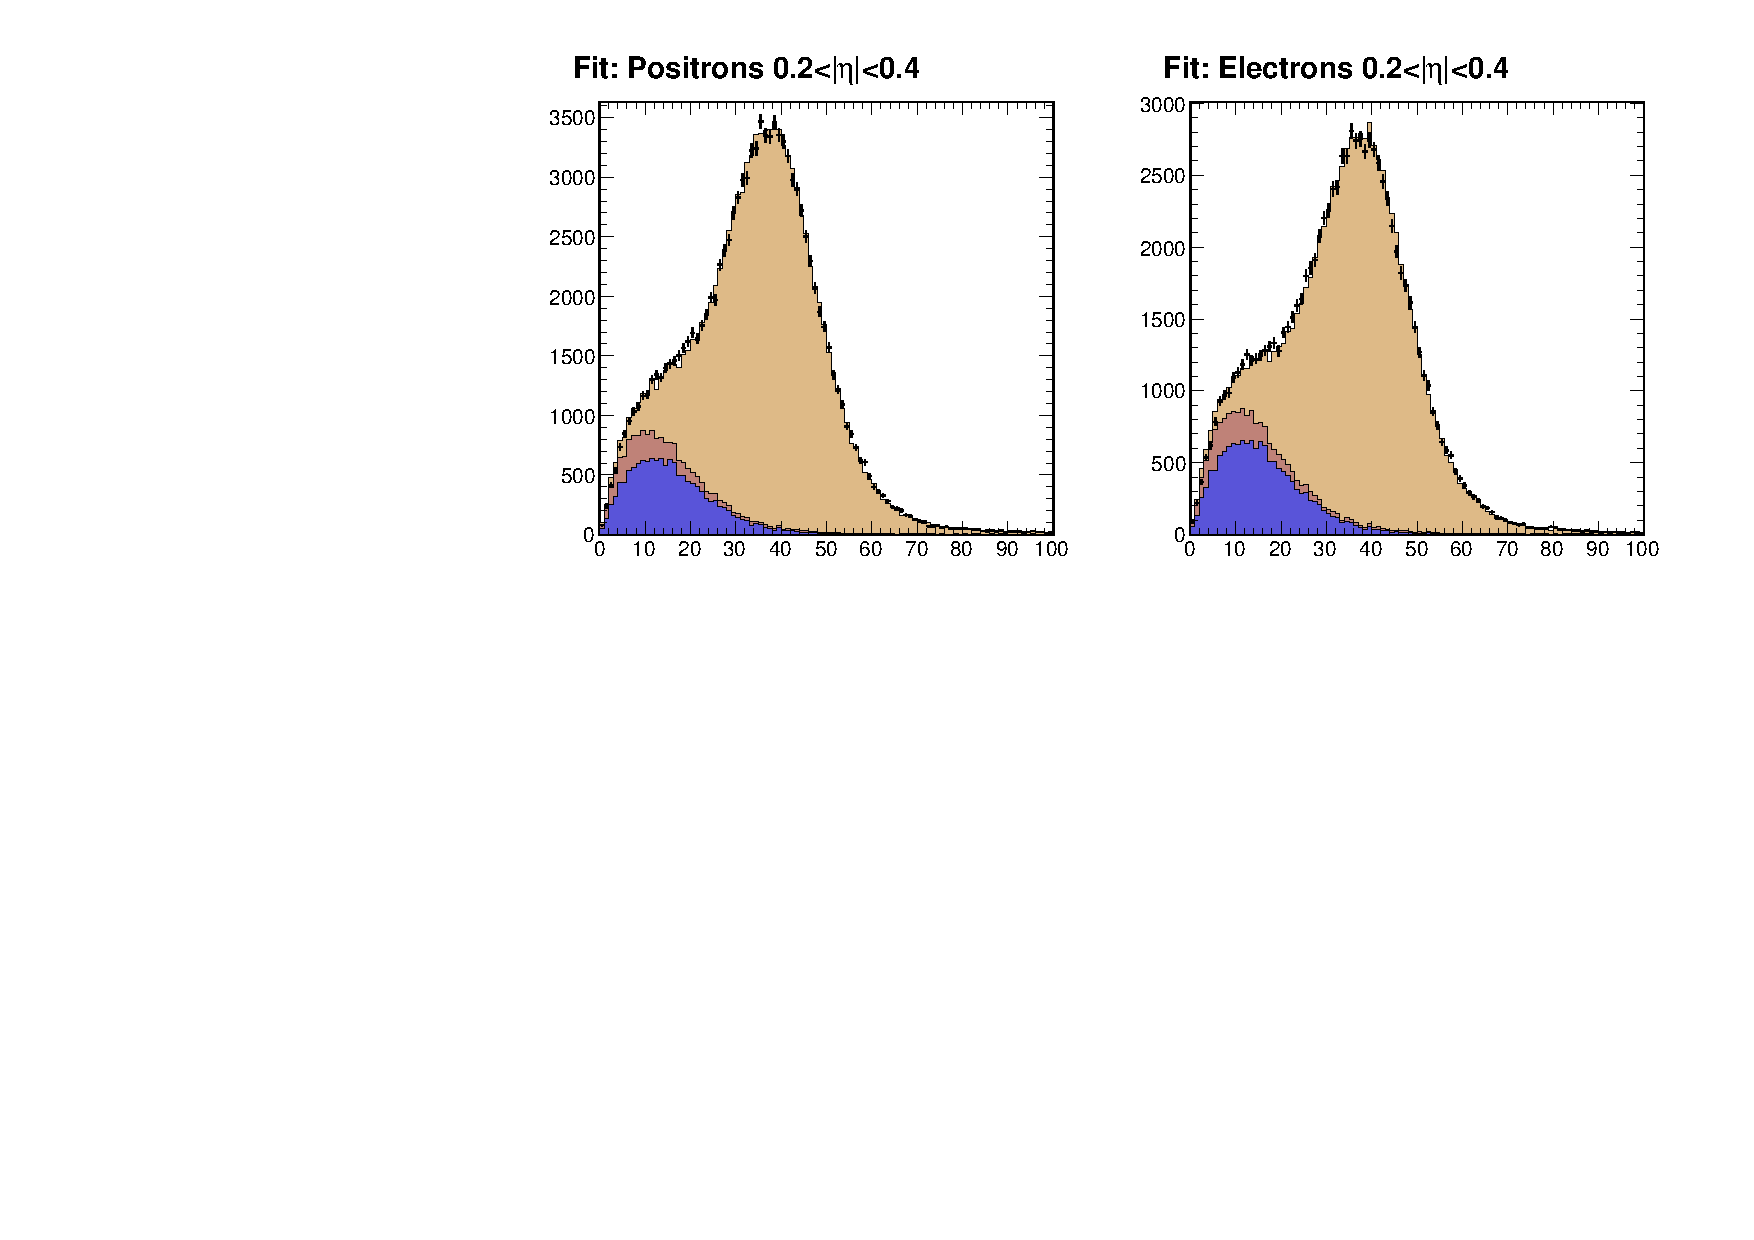
\includegraphics[width=0.95\textwidth]{data_1.pdf} \\
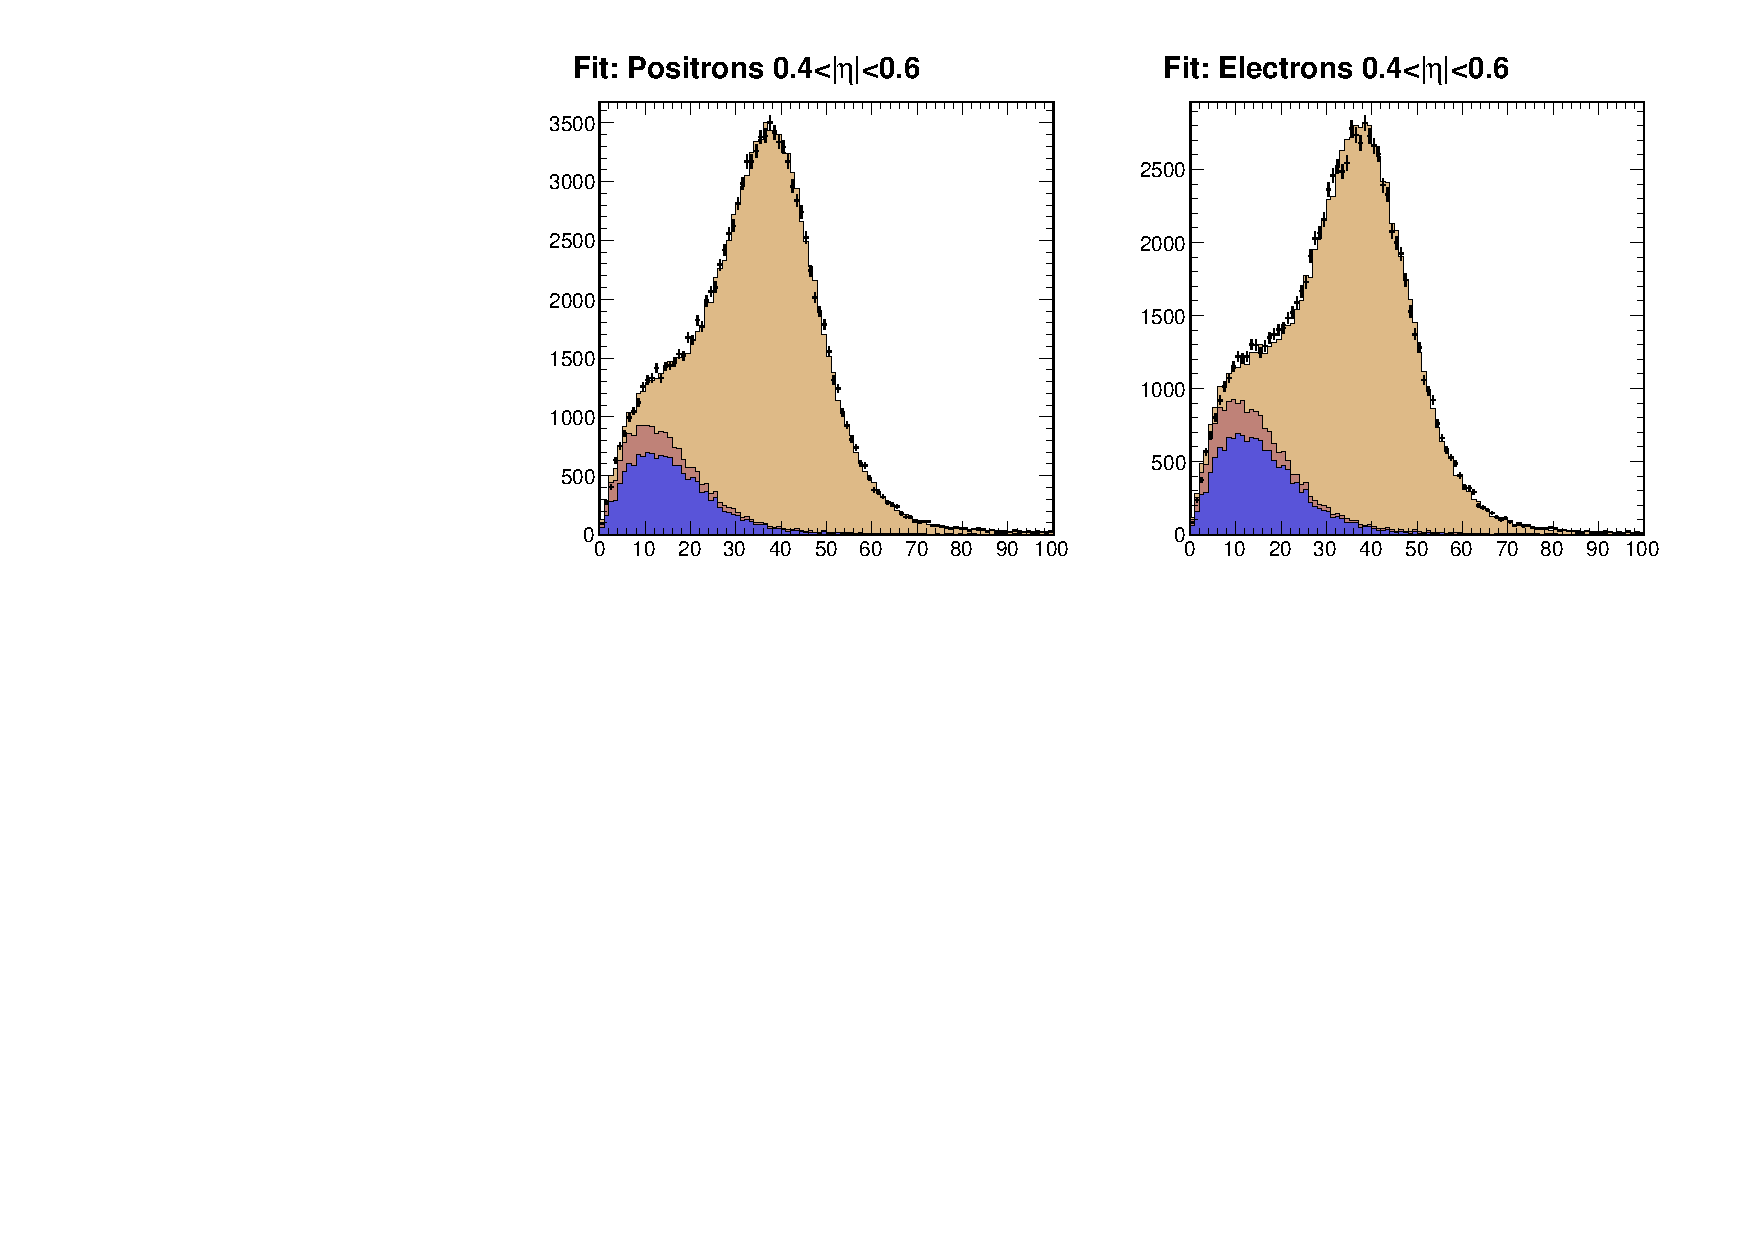
\includegraphics[width=0.95\textwidth]{data_2.pdf}
\caption{  \label{fig:data1} The fit to \MET\ for pseudorapidity bins 1,2 and
3.  The $x$-axis is the particle flow \ETm (GeV) and the $y$-axis is the number
of events ($\GeV^{-1}$).}
\end{center}
\end{figure}

\begin{figure}
\begin{center}
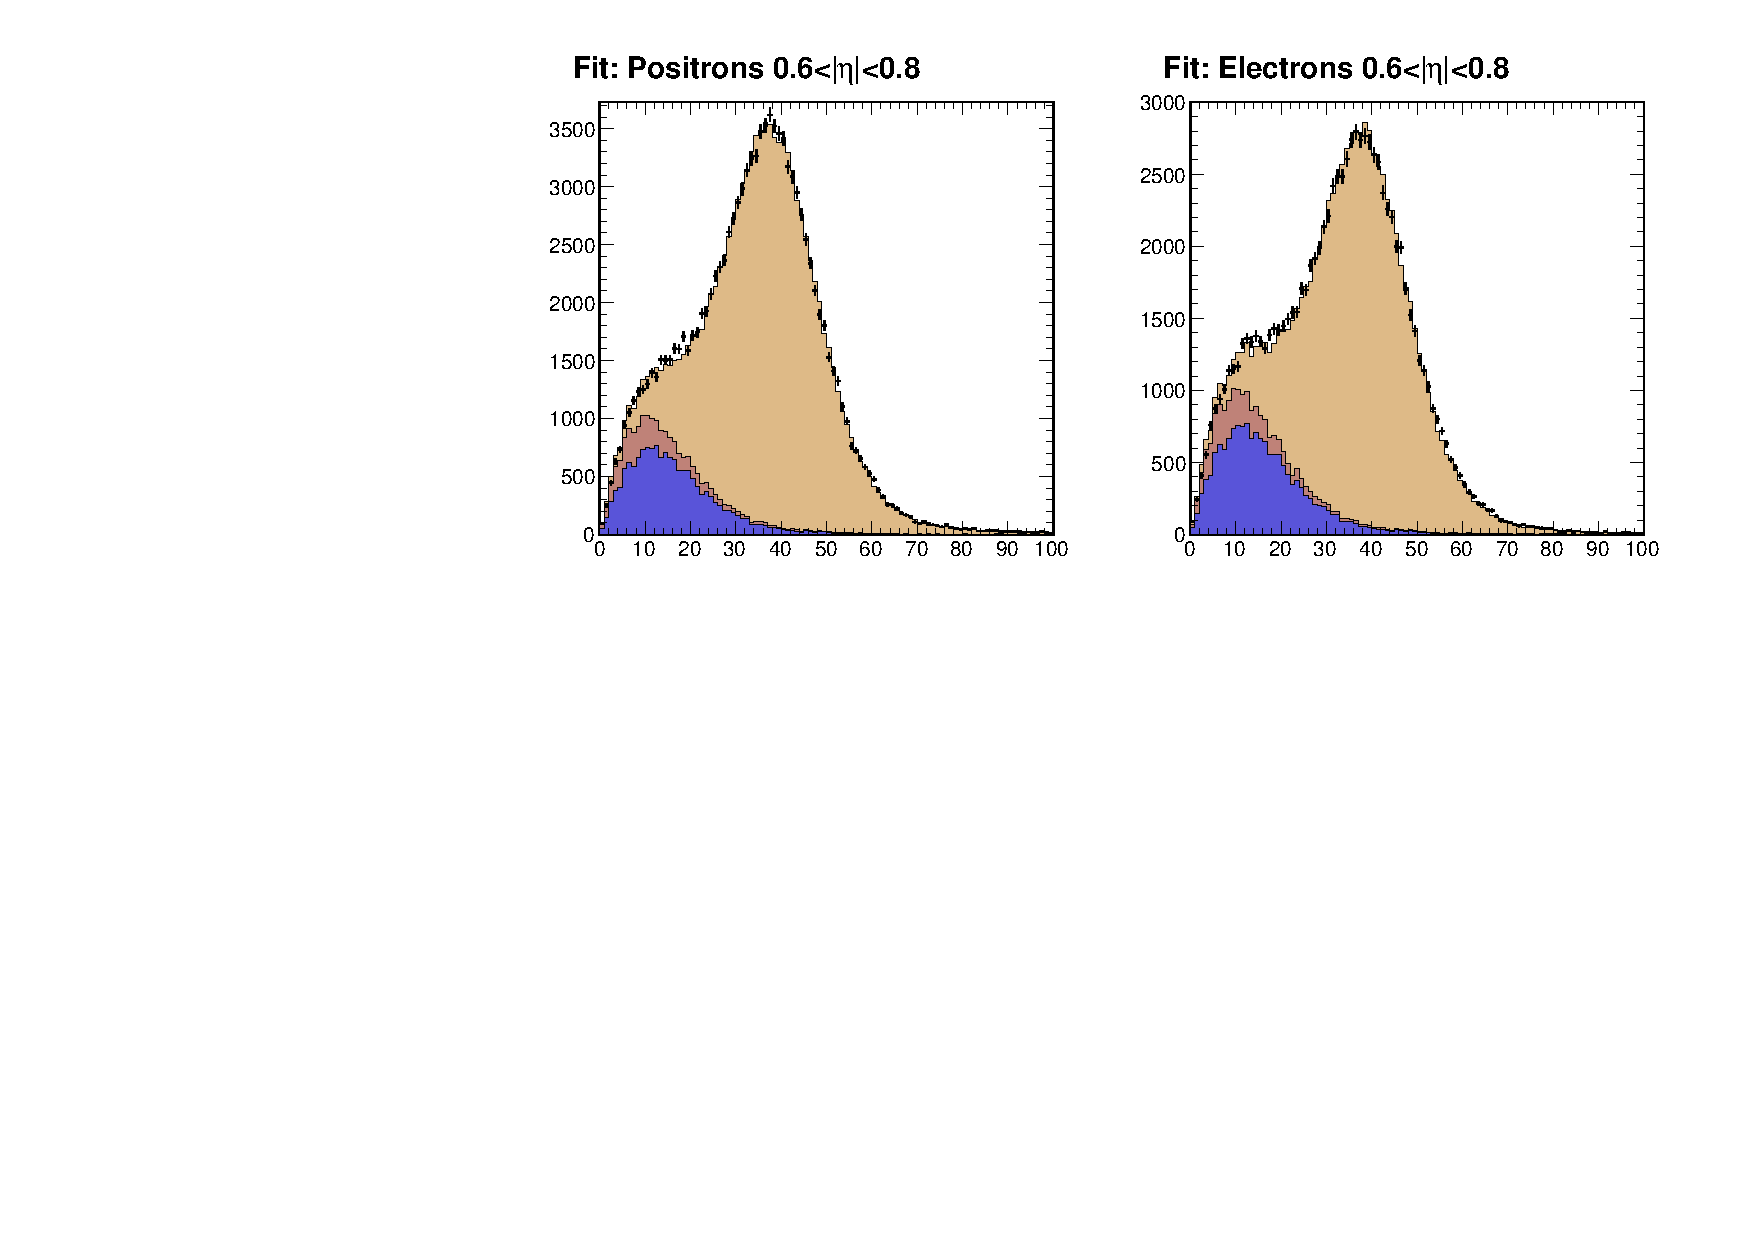
\includegraphics[width=0.95\textwidth]{data_3.pdf} \\
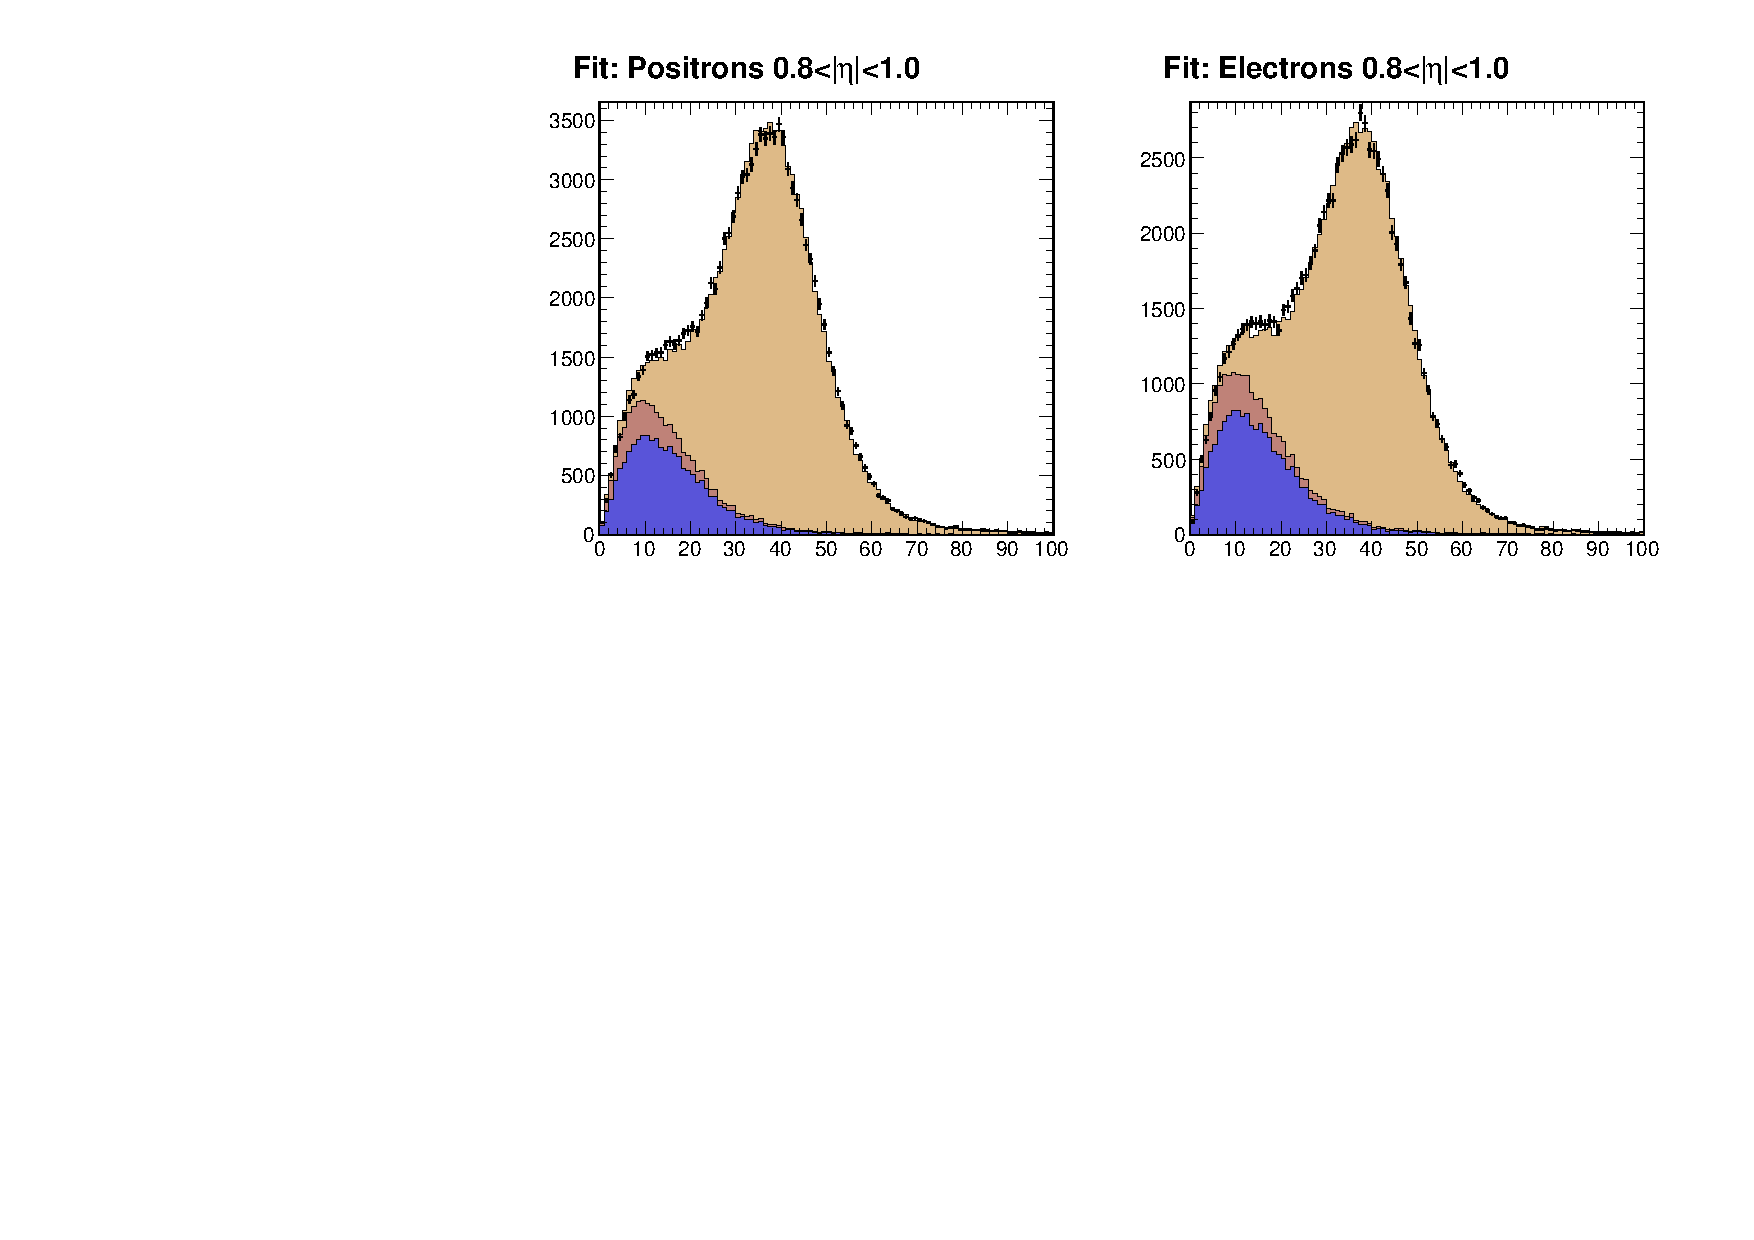
\includegraphics[width=0.95\textwidth]{data_4.pdf} \\
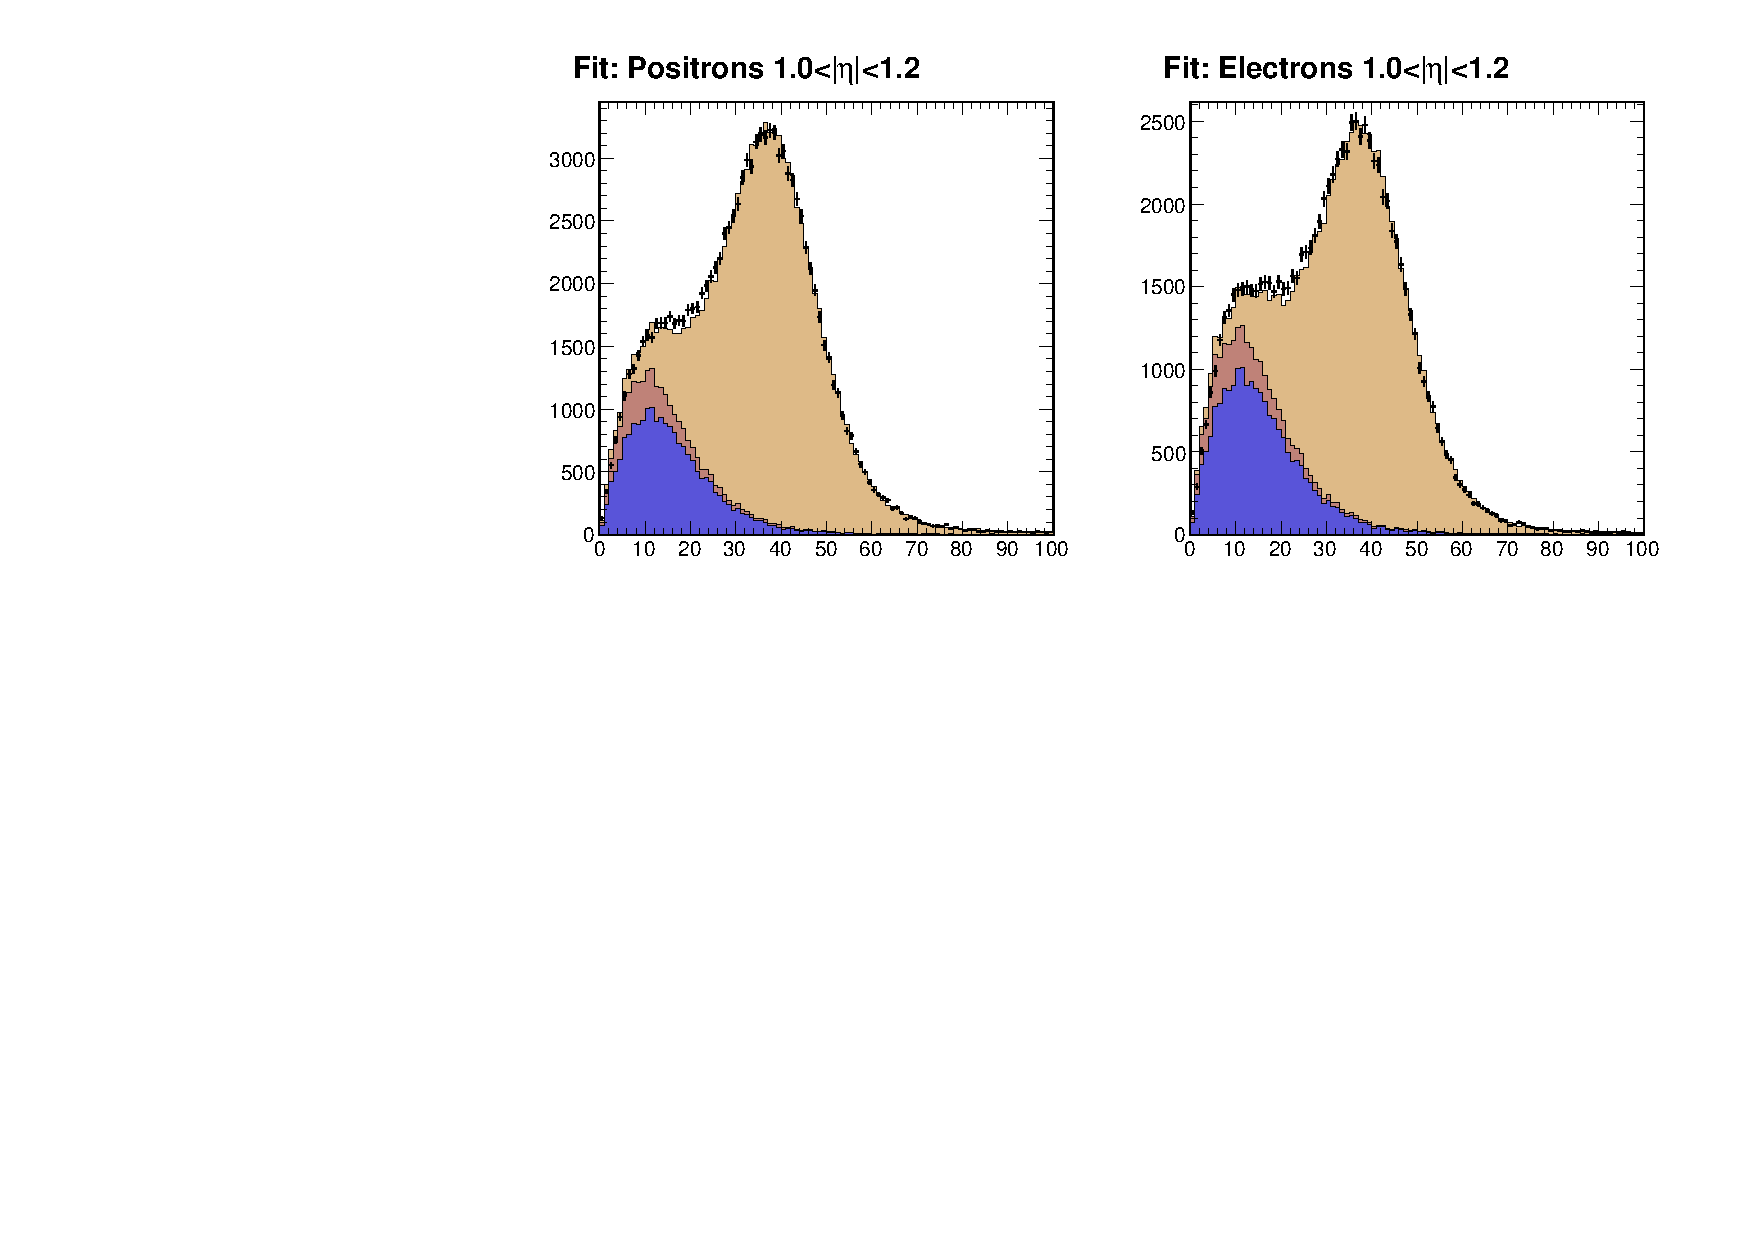
\includegraphics[width=0.95\textwidth]{data_5.pdf}
\caption{  \label{fig:data2} The fit to \MET\ for pseudorapidity bins 4,5 and
6.  The $x$-axis is the particle flow \ETm (GeV) and the $y$-axis is the number
of events ($\GeV^{-1}$).}
\end{center}
\end{figure}

\begin{figure}
\begin{center}
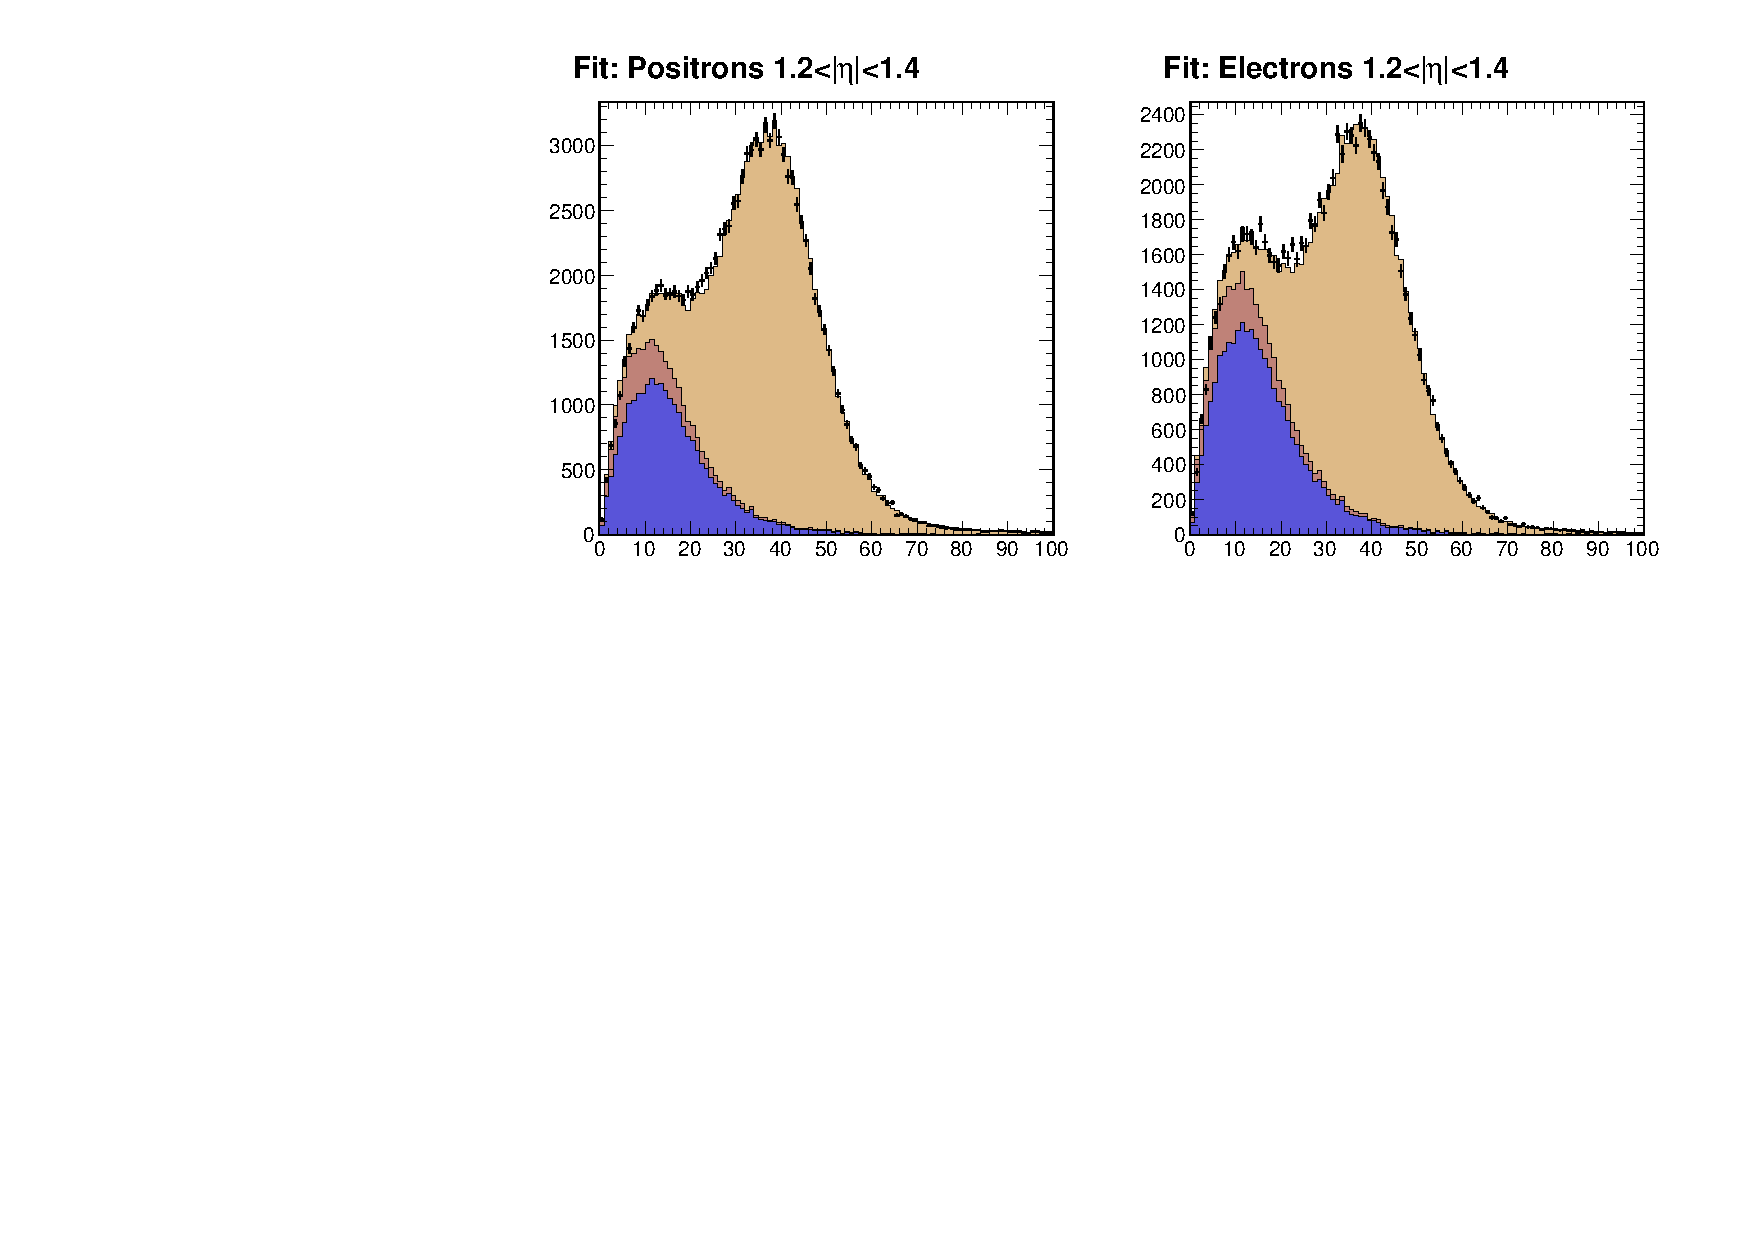
\includegraphics[width=0.95\textwidth]{data_6.pdf} \\
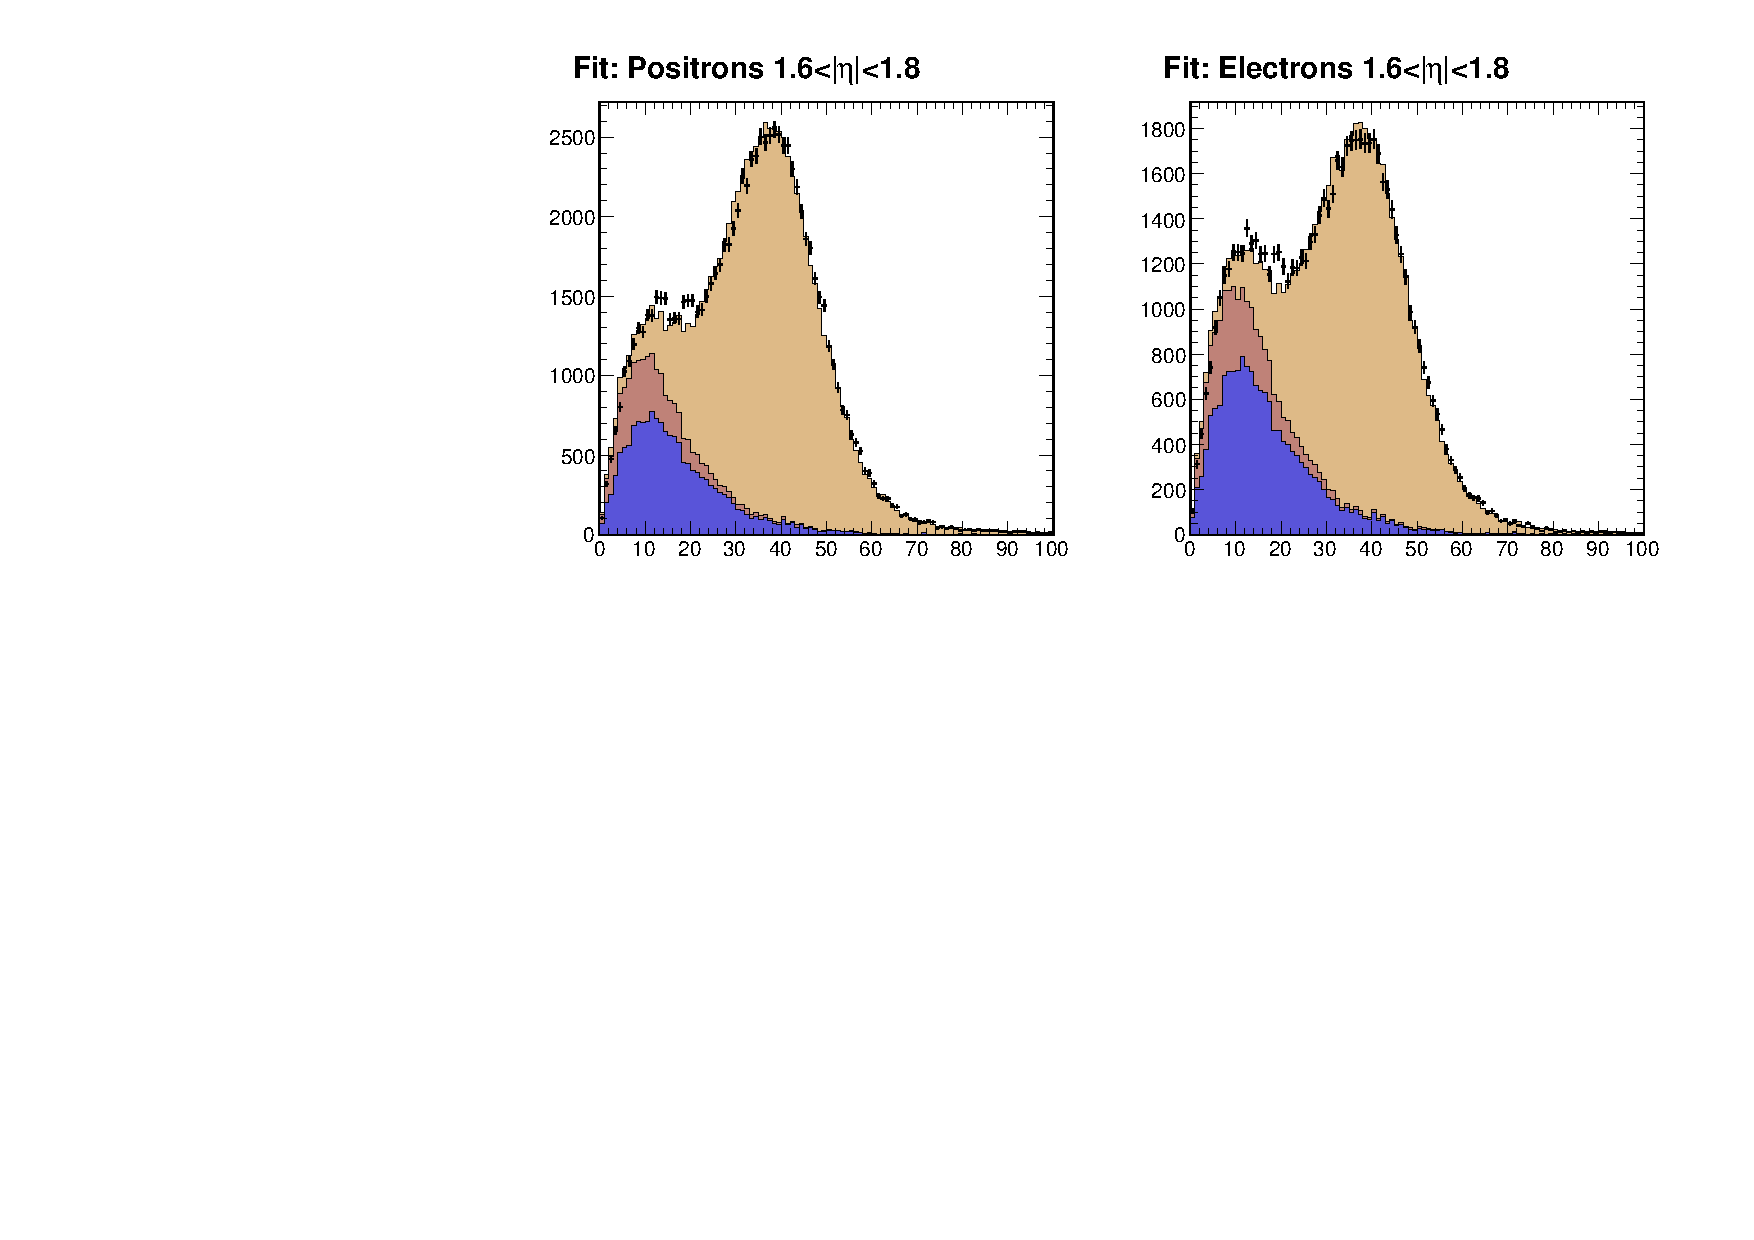
\includegraphics[width=0.95\textwidth]{data_7.pdf} \\
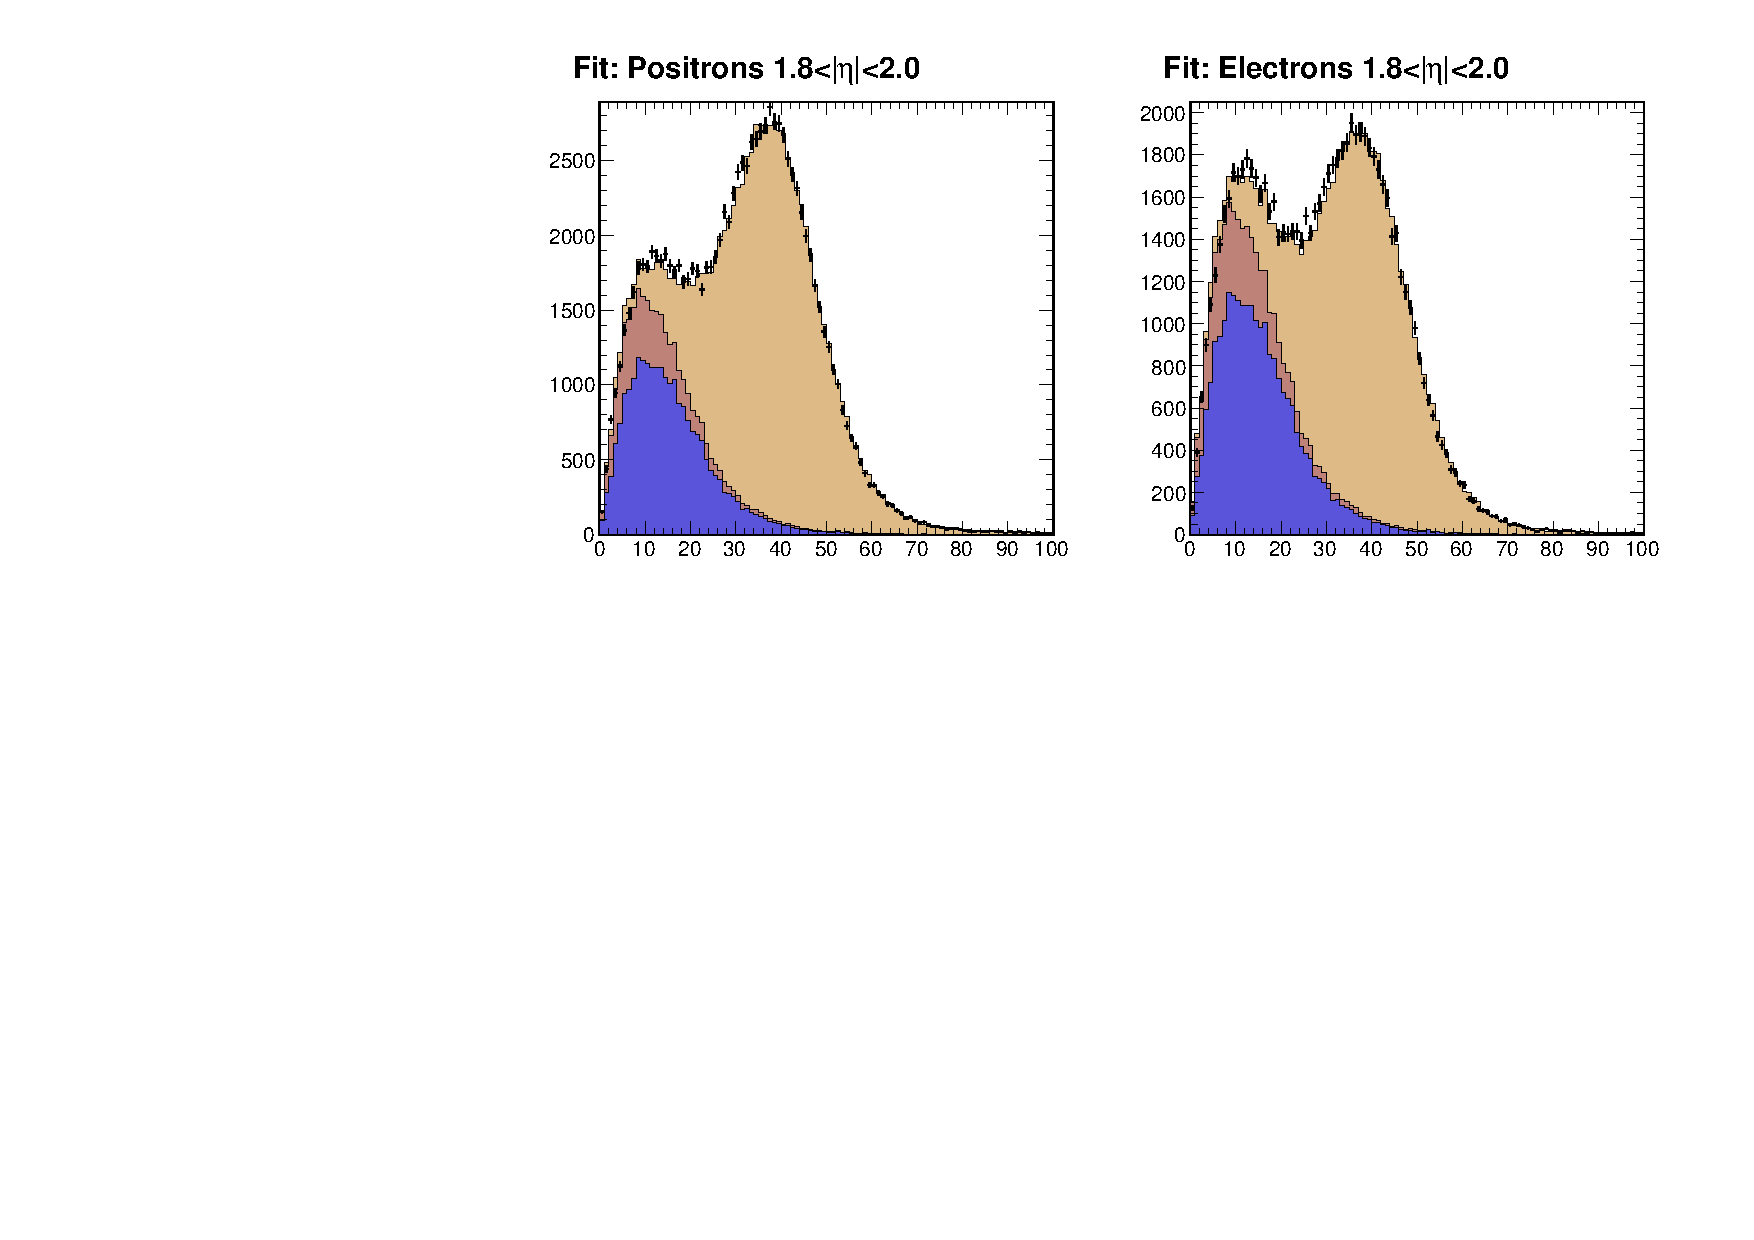
\includegraphics[width=0.95\textwidth]{data_8.pdf}
\caption{  \label{fig:data3} The fit to \MET\ for pseudorapidity bins 7,8 and
9.  The $x$-axis is the particle flow \ETm (GeV) and the $y$-axis is the number
of events ($\GeV^{-1}$).}
\end{center}
\end{figure}

\begin{figure}
\begin{center}
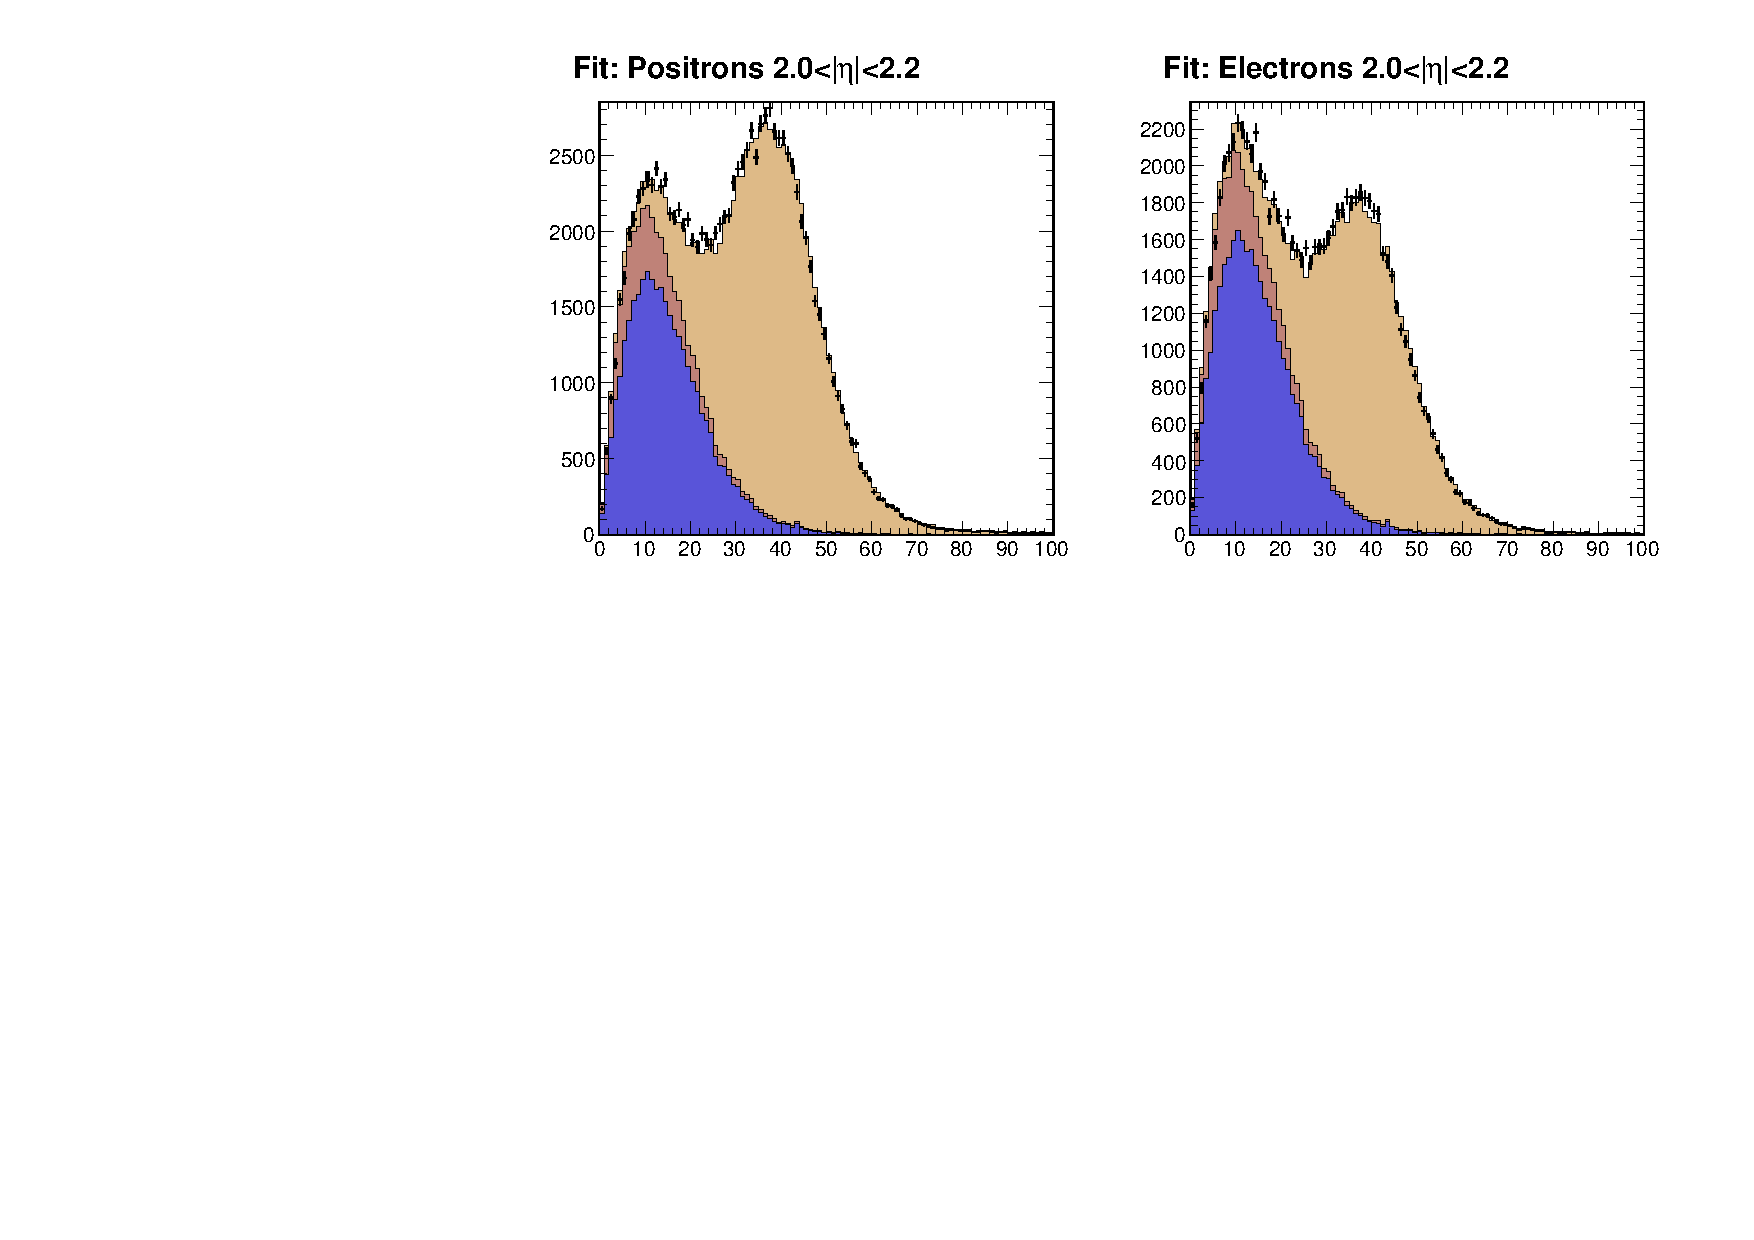
\includegraphics[width=0.95\textwidth]{data_9.pdf} \\
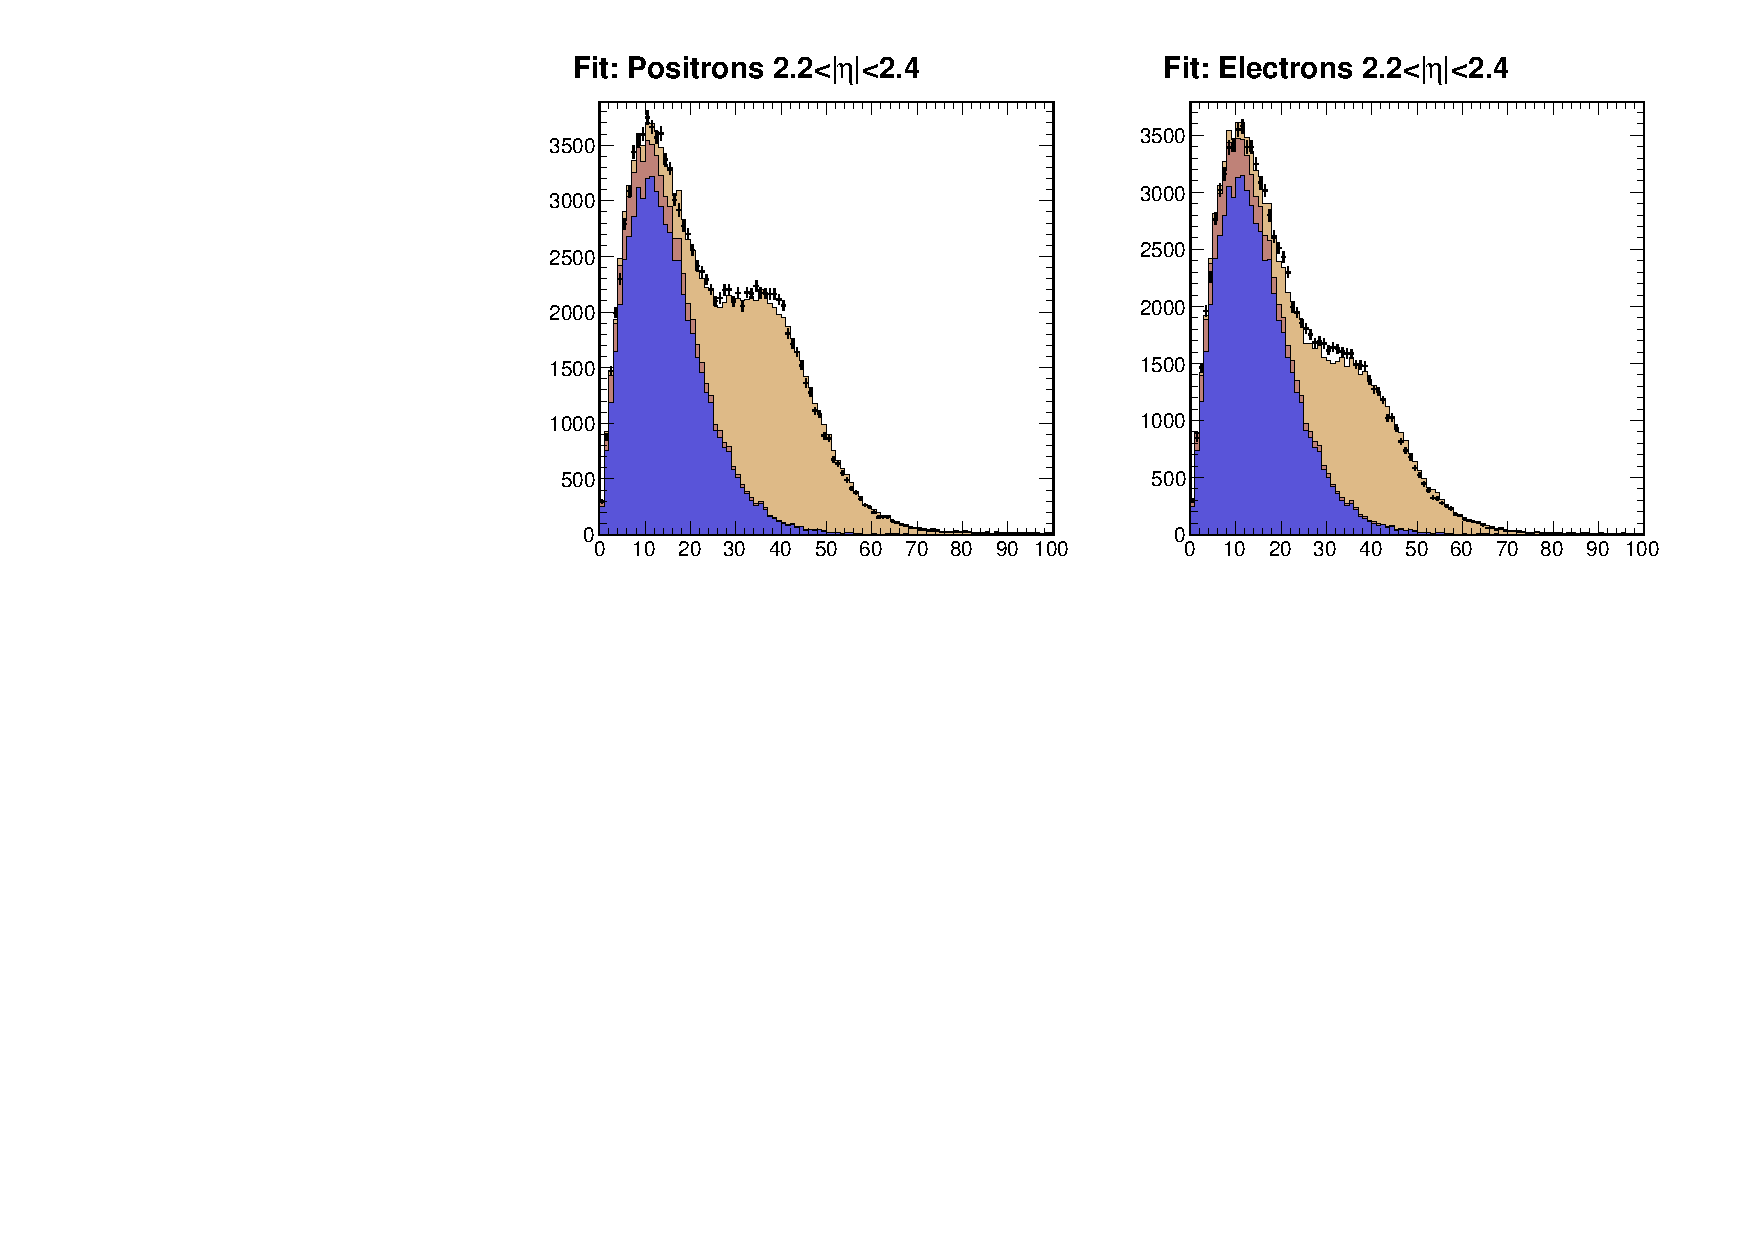
\includegraphics[width=0.95\textwidth]{data_10.pdf}
\caption{  \label{fig:data4} The fit to \MET\ for pseudorapidity bins 10 and
11.  The $x$-axis is the particle flow \ETm (GeV) and the $y$-axis is the number
of events ($\GeV^{-1}$).}
\end{center}
\end{figure}

